% siminos/blog/dailyBlogBB.tex
% $Author: predrag $ $Date: 2017-03-15 15:55:02 -0400 (Wed, 15 Mar 2017) $
% Predrag moved reducesymm/blog/dailyBlogBB.tex to here     Nov 15 2013
% Predrag  switched to github.com                           Jul  8 2013
%           continues siminos/blog/dailyBlog.tex as of that date

\chapter{Burak's notes}
\label{c-dailyBlogBB}

\renewcommand{\LieEl}{\ensuremath{g}}  % Predrag Lie group element
\renewcommand{\gSpace}{\ensuremath{\theta}}   % group rotation parameters
\renewcommand{\ssp}{x}
\renewcommand{\sspRed}{\ensuremath{\hat{x}}}  % reduced state space point
\renewcommand{\vel}{\ensuremath{v}}   % state space velocity

\begin{description}

\item[2014-02-08  Predrag] \refSect{sect-SinglSlice} is a staging ground
for \texttt{siminos/slice/slice.tex}
\HREF{../slice/slice.pdf} {PRLett draft}.

\end{description}

\section{A single slice hyperplane for \SOn{2}}
\label{sect-SinglSlice}


We show how to the  reduce \SOn{2}\ symmetry for PDEs on periodic
domains, for example \KS\ equation, using a single \slice\ hyperplane.
The method is an implementation of Ruslan Davidchack's 2007
proposal\rf{Davidchack_priv} that for \KS\ the \slice\ condition be
imposed by fixing the first Fourier mode, augmented by a time rescaling
that speeds up numerical integrations of the equations of motion for such
problems.

Consider a Fourier
series expansion of a real-valued smooth periodic function:
\beq
	u(\phi) = a_0 + \sum\limits_{k=- \infty}^\infty a_k e^{i k \phi} .
\ee{FourierSeries}
Truncating the expansion to $m$ modes we
write the real and imaginary parts of the Fourier coefficients with
$k \geq 1$ in a state vector $(b_1, c_1, b_2, c_2,..., b_m, c_m)$, where
$a_i = b_i + i c_i$, and $\SOn{2}$ acts on this vector
as a block diagonal rotation matrix,
\beq
	\LieEl(\theta) = \begin{pmatrix}
						R(\theta) & 0 			  & \cdots & 0 \\
						0		   & R(2 \theta) & \cdots & 0 \\
						\vdots	   & \vdots 	  & \ddots & \vdots \\
						0		   & 0	          & \cdots & R (m \theta)
					   \end{pmatrix}
\,,\quad %\beq
	R(k \theta) =	\begin{pmatrix}
					\cos k \theta & \sin k \theta \\
					-\sin k \theta & \cos k \theta
					\end{pmatrix}
\,,
\ee{eq:SO2rotMat}
with Lie algebra generator
\beq
	\Lg  = \begin{pmatrix}
						T & 0 			  & \cdots & 0 \\
						0		   & 2T & \cdots & 0 \\
						\vdots	   & \vdots 	  & \ddots & \vdots \\
						0		   & 0	          & \cdots & mT
					   \end{pmatrix}
\,,\quad %\beq
	         T =	\begin{pmatrix}
					 0 & 1 \\
					-1 & 0
					\end{pmatrix}
\,.
\ee{eq:LgSO2}
Now let us consider the following specific choice of a \slice\ \template\:
\beq
	\slicep = (1, 0, ..., 0) .
\ee{firstmodetemp}
The \slice\ condition
\beq
\braket{\sspRed(t) - \slicep}{\sliceTan{}}
= \braket{\sspRed(t)}{\sliceTan{}}
= 0
%\,.
\ee{SliceCond}
restricts the points in the \slice\ hyperplane defined
by the template point \refeq{slicetemp} of form
\beq
	\sspRed = (\hat{b}_1, 0, \hat{b}_2, \hat{c}_2, ..., \hat{b}_m, \hat{c}_m) .
\ee{slicetemp}
These points satisfy the \chartBord\ condition
\beq
\braket{\groupTan(\sspRed^*)}{\sliceTan{}} = 0
\,.
\ee{ChartBordCond}
only if $\hat{b}_1 = 0$, in other words, as long as the first mode
magnitude is non zero, there is a corresponding unique point to every
group orbit on the \slicePlane\ defined by \refeq{firstmodetemp}. By
rotational invariance, any  \template\ point of form
$\slicep=\{\sin\phi,\cos\phi,0,0,\cdots,0\}$ in the first Fourier mode
plane would do as well since the first mode has the symmetry of a circle;
we pick the \slice\ \template\ \refeq{firstmodetemp} for computational
convenience.

Every group orbit pierces the \slicePlane\ twice. The \slice, however, is
the half-space $b_1 > 0$, up to the \chartBord, pierced  once by any full
\statesp\ group orbit. Invariant subspaces all lie in the \chartBord.

Consider an $m$-mode $\SOn{2}$-equivariant system with the Lie algebra
generator \refeq{eq:LgSO2}.
We assume that there is no $k=0$ Fourier mode,
and that for each $k$ the $k$th Fourier mode appears only once.
    \PC{Recheck: is assuming that $a_0(t)=0$ is really necessary?
    Only equations with Galilean invariance have that...}
    \BB{2014-02-09}{
    This could actually be a real problem, $a_0(t) \neq 0$ can mess things
    up just as $z$ does in \cLe.}
Both assumptions are violated, for example, by the \cLe, where $k=1$
appears twice, but satisfied by \KS,
where $k=0$ Fourier mode vanishes by Galilean invariance, and no
Fourier mode is degenerate.
Let $\slicep$ be a \slice\ template and  $\sspRed^{*}$ be a point on its
\chartBord. The \slice\ \refeq{SliceCond} and \chartBord\
\refeq{ChartBordCond} conditions take form
    \PC{sorry, this is a repeat of the argument above: need to condense}
\begin{subequations}\label{eq:mmodechartbord}
\begin{align}
	\sum_{k=1}^{m} k  (\sspRed_{2k-1}^{*} \slicep_{2k}
                       - \sspRed_{2k}^{*} \slicep_{2k-1})&= 0 ,
	\label{eq:mmodechartborda}
\\
	\sum_{k=1}^{m} k^2 (\sspRed_{2k-1}^{*} \slicep_{2k-1}
                       + \sspRed_{2k}^{*} \slicep_{2k}) &= 0
	\label{eq:mmodechartbordb} .
\,,
\end{align}
\end{subequations}
where subscripts denote vector components. If the \slice\ condition
affects only the $k$ Fourier mode, for example, for
$\slicep=\{0,0,\cdots,1,1,0,0,\cdots,0\}$, \refeq{eq:mmodechartbord} reduces to:
\begin{subequations}\label{eq:mmodechartbordred}
\begin{align}
	\sspRed_{2k-1}^{*} - \sspRed_{2k}^{*} &= 0 ,
	\label{eq:mmodechartbordreda}
\\
	\sspRed_{2k-1}^{*} + \sspRed_{2k}^{*} &= 0 .
	\label{eq:mmodechartbordredb}
\end{align}
\end{subequations}
The $d=2m$\dmn\ point $\sspRed^{*}$ lies in the
\chartBord\ only if the $k$th Fourier mode vanishes,
$\sspRed_{2k-1}^{*} = \sspRed_{2k}^{*} = 0$. We shall
assume that a generic `turbulent' state
of the system has vanishing probability that its $k$th Fourier mode
is exactly 0. An ergodic orbit will pass arbitrarily close to
the
\chartBord\ arbitrarily often, but never penetrate it, and thus never cross
it.
    \PC{2014-02-22 Evangelos and Burak have disproved the claim: ``This
    cannot happen for a generic state of the system, as vanishing k = 0
    Fourier mode is an invariant subspace, which a generic state cannot
    enter or exit.'' {\bf Evangelos}: This depends on the nonlinear
    coupling of Fourier modes. For \twomode\ flow it is true, but not for
    KS, as is clear from the form of $\dot{a}_k$ for $a_k=0$. }
Thus, it is possible to reduce globally the symmetry of an $m$-modes
$\SOn{2}$-equivariant system using a template $\slicep$ which fixes the
phase of $k$th Fourier mode, as long as both $k$th mode amplitudes never
vanish simultaneously.
    \PC{2014-02-22 this was wrong, removed: ``If $k=1$ Fourier mode
    vanishes, we are within the \chartBord\, and studying dynamics in an
    invariant subspace where $k=2$ Fourier mode needs to be fixed, and so
    on. See Ruslan's discussion in \refsect{2009-08-29KS-O2}.''}
Choosing which Fourier mode phase might depend on the dynamics.
For a small, $L=22$ \KS\ system\rf{SCD07} the dynamics is dominated by the
competition of the 2nd and 3rd Fourier modes, so fixing the phase of
the $k=2$, $k=3$
or $k=6$ mode might be preferable to fixing the phase
of the longest wavelength but dynamically less prominent $k=1$ mode.
This is illustrated by \reffig{fig:BBKShigherFmode}.

For \SOn{2} the symmetry-reduced dynamics $\sspRed (t)$ and the
time dependent group parameter $\theta (t)$ are obtained by integrating
the equations in the \slice:
\bea
\velRed(\sspRed) &=& \vel(\sspRed)
   -\dot{\gSpace}(\sspRed) \, \groupTan(\sspRed)
\continue
\dot{\gSpace}(\sspRed) &=& {\braket{\vel(\sspRed)}{\sliceTan{}}}/
               {\braket{\groupTan(\sspRed)}{\sliceTan{}}}
\,.
\label{eq:so2reduced}
\eea
Here, $\velRed$ is the component of the velocity field in the \slicePlane.

%%%%%%%%%%%%%%%%%%%%%%%%%%%%%%%%%%%%%%%%%%%
\begin{figure}%[H]
\centering
 (a) 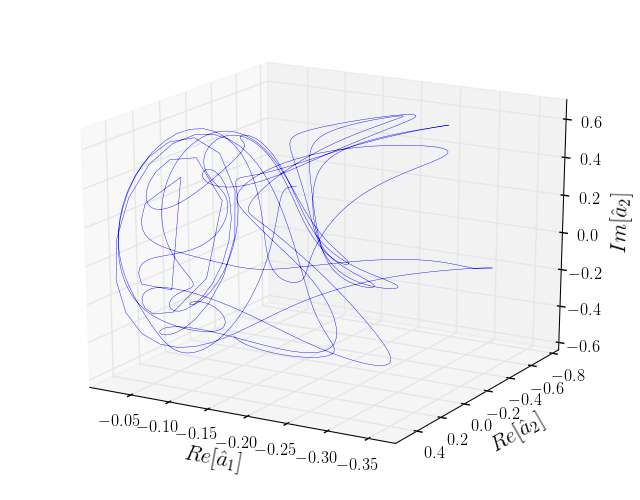
\includegraphics[width=0.45\textwidth]{BBKSmovframes}
 (b) 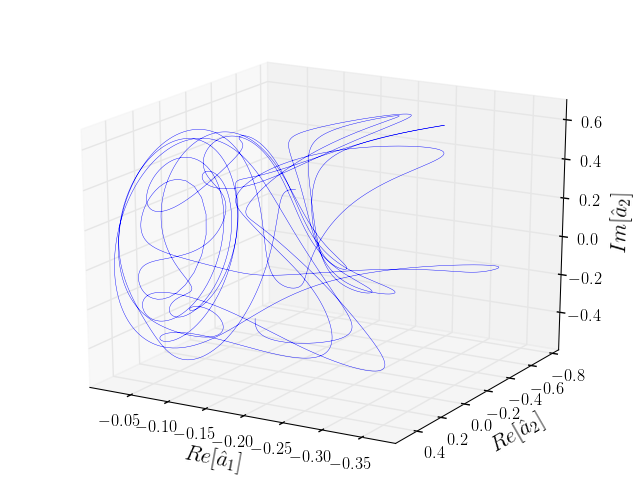
\includegraphics[width=0.45\textwidth]{BBKSmovframesb}
\caption{
The single-\slicePlane\ symmetry reduced \KS\ flow with
(a)  integration time step $\Delta t = 0.1$
exhibits large jumps close to the {\chartBord};
(b) with integration time step $\Delta t = 0.01$ is smooth.
}
\label{fig:BBKSmovframes}
\end{figure}
%%%%%%%%%%%%%%%%%%%%%%%%%%%%%%%%%%%%%%%%%%%

%%%%%%%%%%%%%%%%%%%%%%%%%%%%%%%%%%%%%%%%%%%
\begin{figure}%[H]
\centering
% (a) 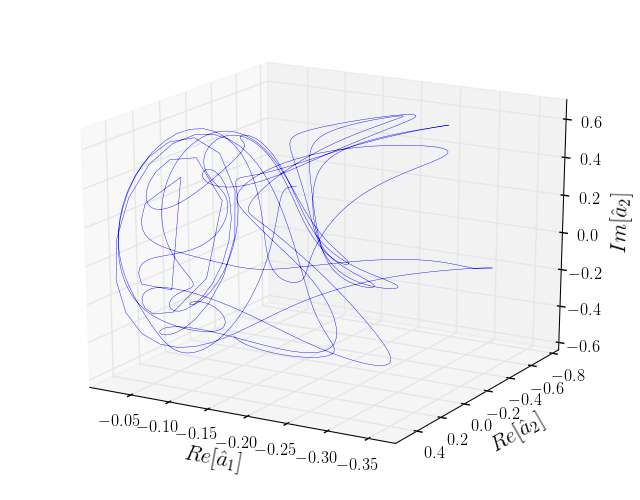
\includegraphics[width=0.45\textwidth]{BBKSmovframes}
% (b) 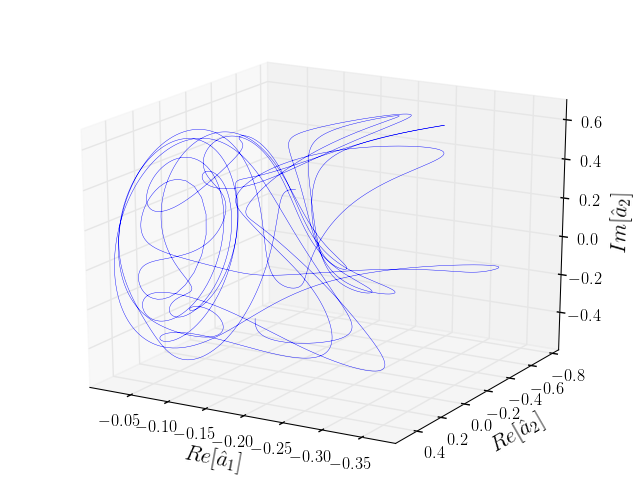
\includegraphics[width=0.45\textwidth]{BBKSmovframesb}
\caption{
The $k$th mode \slicePlane\ symmetry-reduced \KS\ flow with
(a)  $k=2$,
(b) $k=3$,
(c) $k=6$,
in the time / configuration space $\hat{u}(x,\zeit)$ representation,
and
various \statesp\ representations.
}
\label{fig:BBKShigherFmode}
\end{figure}
%%%%%%%%%%%%%%%%%%%%%%%%%%%%%%%%%%%%%%%%%%%



The problem with the slice condition is that close to the {\chartBord}
the denominator $\braket{\groupTan(\sspRed)}{\sliceTan{}}$, can be small,
and the {\phaseVel} ${\gSpace}$, can vary rapidly, necessitating
numerical integration with small time steps, as illustrated in
\reffig{fig:BBKSmovframes}. However, if we rescale the time parameter as
$d\tau = b_1 dt$
  \ES{I think you meant to write $dt=b_1 d\tau$. }
  \BB{2014-02-09}{Yes, thanks.}
given the first Fourier mode \slice\ condition $\slicep
= (1,0,0,0,...)$, the dynamics \refeq{eq:so2reduced} in the \slice\ takes
form:
\bea
\frac{d \sspRed}{d \tau} &=& \sspRed_1 \vel(\sspRed)
   - \frac{d \gSpace(\sspRed)}{d \tau} \, \groupTan(\sspRed)
\continue
\frac{d \gSpace(\sspRed)}{d \tau} &=& -\vel(\sspRed)_2
\,.
\label{eq:scaledtime}
\eea
The single {\slicePlane} construction guarantees that $b_1>0$, so the
rescaled time has the same sign as the original time. As this is only a
reparametrization of orbits, \ie, 1D curves swept out by dynamics, the
original \refeq{eq:so2reduced} and the rescaled \refeq{eq:scaledtime}
have the same invariant solutions, the only thing that differs are the
`time tics' along the curves. The velocity $\vel(\ssp)_2$, \ie, the rate
of change of the first Fourier mode is typically a smooth, nonsingular
function, so in the rescaled time there are no rapid  {\phaseVel}
variations close to the {\chartBord}, and no variable time-step
refinements are needed for numerical integrators.

In particular, if Kimberly and Ashley redo their computations of
$\dot{\gSpace}$, in the rescaled time there should be no wild
oscillations that they see in the original time, and recurrence plots
should be much healthier.

And to Xiong Ding and Adam Fox: start working in the symmetry-reduced
\KS\ \statesp, there is no excuse not to do it.

%%%%%%%%%%%%%%%%%%%%%%%%%%%%%%%%%%%%%%%%%%%%%%%%%%%%%%%%%
\input BudCvi14edits
% Predrag 2014-08-23 separated out \section{BudCvi14 edits}
%%%%%%%%%%%%%%%%%%%%%%%%%%%%%%%%%%%%%%%%%%%%%%%%%%%%%%%%%

%%%%%%%%%%%%%%%%%%%%%%%%%%%%%%%%%%%%%%%%%%%%%%%%%%%%%%%%%
\input BudCvi15edits
% Predrag 2014-08-23 separated out \section{BudCvi15 edits}
%%%%%%%%%%%%%%%%%%%%%%%%%%%%%%%%%%%%%%%%%%%%%%%%%%%%%%%%%

\section{A single slice hyperplane commentary}
\begin{description}

\item[2013-09-10 Burak, 2014-02-07 Burak + Predrag]
I have found a general way of reducing the \SOn{2}\ symmetry for PDEs on
periodic domains using single \slice\ hyperplane, read
\refsect{sect-SinglSlice}.

\item[2013-09-11 Predrag] This, I think, is the first thing we tried,
and what Ruslan believes is the solution, so he has since refused any of
the slicing entanglements that we have developed.
He might well be right - I would love the simplest solution to be the
right one. Read
\refsect{HowtoQuotSO2},
\refsect{2009-08-25Eurosceptics},
\refsect{2009-08-29KS-O2} and so on. Please read those discussions critically.
We did not follow Ruslan's prescription, right or wrong.

At some point, you might want to read / scan through
all 300+ pages of the historical blog, ask me
questions if anything looks different.

\item[2013-09-11 Burak] My single slice argument should work for problems
that are defined on a periodic domain and handled in terms of different
Fourier modes, since, in that case, the \Lg\ can be written in the form
\refeq{eq:LgSO2} and the first Fourier mode is never
zero for a reasonable set up (Right? If the first Fourier mode is zero,
then the second mode is actually the first.).

\item[2013-11-02 Burak] I used Ruslan's solver for \KS\ and got a fairly chaotic
looking trajectory for random initial conditions then sliced it with moving
frames method using $\slicep=\{1,1,0,0,\cdots,0\}$.
Result is in \reffig{fig:BBKSmovframes}. If you look carefully you can see
some discontinuity around $Re[\hat{a}_1] = 0$, that is due to $\dot{\phi}$
being larger around that region and it goes away as you make your timesteps
smaller. In this figure, time step is fixed to $\Delta t = 0.1$, I belive
a solution within the slice that uses adaptive time-stepping can produce much
better results, however, until now, I wasn't successful in numerically solving
\KS\ equation myself.

If you want to produce the \reffig{fig:BBKSmovframes} and rotate it, first
make sure that you have the required packages by running

\texttt{bash DEBIAN.sh} (for Ubuntu and Debian based distros) or

\texttt{bash FEDORA.sh} (for Fedora) in

\texttt{blog/burak/KuramotoShivashinsky/python/}

then run

\texttt{bash solvenslice.sh}

in the same folder. This should generate a Matlab-like rotatable figure.

\item[2013-09-14 Burak]
The reason that I'm sure that single slice would work for \twoMode\ system
has to do with its invariant subspace. In the invariant polynomial basis,
the invariant subspace is $(u,v,w,q) = (0,v,0,0)$ which corresponds to
$(x_1,x_2,y_1,y_2) = (0,0,y_1,y_2)$
in the full state space which is the \chartBord. Hence the dynamics that
would start outside the \chartBord\ will never get into the \chartBord\
in the \twoMode\ system. In other words, in \twoMode\ system, the invariant
subspace is the subspace where the dynamics is confined into the pure $m=2$
Fourier mode. Since the \twoMode\ system is the most general system with
2 Fourier modes, this urges me to check whether a similar statement can
be made in systems with higher Fourier modes. Namely, if we can show that
all invariant subspaces of an m-mode \SOn{2}\ symmetric system will exclude
$m = 1$ region, we can say that an m-mode \SOn{2}\ symmetric system can always
be symmetry reduced using a single slice given by $(1,1,0,0,0,...)$ without
any trouble. I'll be working on this for a while before fixing integration
routines which is a rather more trivial task.

\item[2013-09-29 Burak]
This slice works for any system with \SOn{2} symmetry as long as the
magnitude of the first mode is zero. I, myself, haven't studied KS or NS
in detail, so I don't have a precise argument about possible general use.
However, I intuitively say that if a Fourier expanded solution has no first
mode, then the second mode is the actual first mode and one should redefine
their periodic domain. For the case of KS in periodic domain, if you ignore
the nonlinear part, 1st mode is the slowest vanishing mode, so I am guessing
that this method will work for KS. Please let me know, if there is a KS solution
of interest for which both of the real and positive parts of the first mode
is 0. If there is no such known situation, then there is hope. Also for the
experimental data, if you want to Fourier expand your solutions, you have
the freedom of choosing your domain for periodic functions, so if you choose
your domain properly, this method will work just fine without dealing with
chart borders, ridges etc. If you are sure that 0 1st mode solutions are
there and important, then we can propose another multiple-chart scheme and
say when 1st mode is 0, one should jump to the chart of the smallest non-vanishing
Fourier mode.

\item[2013-09-30 Evangelos]
The template you use gives you a slice that is equivalent to
requiring, e.g. $x_1=0$ (this is a consequence of rotational symmetry of your problem --
you can rotate your template any way you like).
That was the first think we tried for KS, and it failed
because you don't have the nice property of the first Fourier mode subspace being
flow invariant. Trajectories cross the chart borders and you cannot get away by
simply rotating your template, nor by working with higher Fourier modes. I do not
understand what you mean by ``choose your domain properly.'' The problem is not
that some solutions have vanishing first Fourier mode at all times, the problem is
that chart borders are crossed by trajectories.

\item[2014-02-08 Predrag] The rescaled time \refeq{eq:scaledtime} is fine
for numerical integrations. But I had hoped also for coordinate rescaling
that would replace the wild large radius rotations by $\pi$ in
\reffig{fig:BBKSmovframes} and in the \twomode\ model by straight lines
crossing close to the `origin', as in the sketch of the
\HREF{http://www.youtube.com/watch?v=jkNJHfdZzHM} {homework problem} on
rescaling.

A counter argument is given by Burak's spatial representation of
this ``2-modes truncation'' of a PDEe, where passages close to the
{\chartBord} is seen in the full-\statesp\ flow as a `defect', \ie,
these jumps are not artifacts of the slice, but physical.
\ES{cannot find this here. Is it on git? Maybe it's time to bring
everything back to this repository?}

\item[2014-02-09 Evangelos] Regularized slice dynamics \refeq{eq:scaledtime}
are really good news!

Maybe it is worth generalizing \refeq{eq:scaledtime} to any linear slice
by defining the fictitious time
by $dt=|\braket{\groupTan(\sspRed)}{\sliceTan{}}|\, d\tau$, motivated by
\refeq{ChartBordCond} for the chart border. The absolute value should guarantee
that fictitious time does not run backwards. Then the equations in the slice
take the form
\bea
\frac{d \sspRed}{d \tau} &=& |\braket{\groupTan(\sspRed)}{\sliceTan{}}|\, \vel(\sspRed)
   - \frac{d \gSpace(\sspRed)}{d \tau} \, \groupTan(\sspRed)
\continue
\frac{d \gSpace(\sspRed)}{d \tau} &=& |\braket{\groupTan(\sspRed)}{\sliceTan{}}|\,
		      {\braket{\vel(\sspRed)}{\sliceTan{}}}/
				    {\braket{\groupTan(\sspRed)}{\sliceTan{}}}
\,.
\label{eq:scaledtimeGeneral}
\eea
which is still simple enough.
Although such a generalization does not seem crucial
for the two modes system, I think we may need it for KS where my experience is
that even if you remove the singularity of first mode slice with
less elegant means\rf{SiminosThesis}, you still have problems with the fact
that equilibria $E_2$ and $E_3$ are mapped to the origin and it is very
hard to make sense of \rpo s in their neighborhood.

Burak do you think you could try \refeq{eq:scaledtimeGeneral} with a slice like
$(1,0,1,0)$ for the two modes system, see if you get something reasonable?

\item[2014-02-09 Burak] I think I tried $(1,0,1,0)$ \slice\ for \twoMode\
system and did not get something reasonable but it was a long time ago and
I may have make infinite number of other mistakes when I tried that, so I'll
redo it. There is one important thing about this single \slice\ argument,
that is the \slice\ hyperplane defined by $\slicep = (1,0,0,0)$ satisfies
$x_2 = 0$ and $x_1 > 0$ and the \chartBord\ is at $x_1 = 0$,
so that's why you just can't ``cross'' it. Worst thing that can happen is
you can ``touch'' but cannot go to the other side of the border. I can't
immediately see such a feature for $(1,0,1,0)$ but there can be. If we can
show such property, then may be $(1,0,1,0,1,0,...)$ could be the correct way
to go in general. To check that I did a quick moving frames run for $(1,0,1,0)$
\slice\ in \twoMode\ system and what I got is \reffig{fig:PKmovingframes1010}.
You can see jumps between two sides of the \chartBord . I don't know if
rescaling time can solve that may be it can.

\item[2014-02-09 Evangelos] I do not know either if rescaling time will help,
but it is worth trying in a pathological case like this. If time rescaling helps
also here, then it would be of even greater value! By the way, did you remember
to rotate the initial point on the slice before starting integration? (that's
a common pitfall).

\item[2014-02-09 Burak] \textbf{A question to \KS\ experts:} As far as
I know, current \KS\ solvers you use are based on \texttt{ETDRK4} algorithm.
I briefly read the references and saw they start with assuming linear and
nonlinear parts of the problem at hand is separable. The formula \refeq{eq:scaledtime}
makes \KS\ equation completely non-linear, modes mix in both terms of the
velocity in the \slice\ hyperplane. Do you think \texttt{ETDRK4} would still
be useful or we should look for another solution? I, by the way, tried integrating
\KS\ using build in \texttt{odepack} solvers in \texttt{scipy.integrate}
but both in full \statesp\ and within the \slice\ I got convergent, boring
trajectories.

\item[2014-02-09 Evangelos] That's correct, you cannot use \texttt{ETDRK4}
or integrating factor methods if the stiff part is not linear. Probably introducing
nonlinear through time rescaling does not help with stiffness, so you would need
some other method for stiff systems such as implicit methods.

\item[2014-02-09 Ruslan] I think integrating ODEs on the slice is a bad idea.
I'm sorry I haven't been following this in detail, but why do you need to do it?
Why not just solve the full KSE and then pull the solution onto the slice?
What are you going to get with integrating on the slice that you
are not getting with integrating the full KS flow?

%%%%%%%%%%%%%%%%%%%%%%%%%%%%%%%%%%%%%%%%%%%
\begin{figure}%[H]
 \centering
 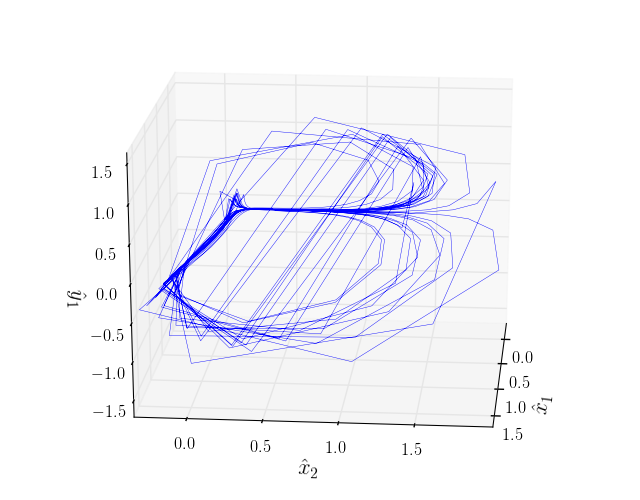
\includegraphics[width=0.6\textwidth]{PKmovingframes1010}

\caption{\twoMode\ dynamics in $(1,0,1,0)$ slice}

\label{fig:PKmovingframes1010}
\end{figure}
%%%%%%%%%%%%%%%%%%%%%%%%%%%%%%%%%%%%%%%%%%%


\item[2014-02-08 Predrag] As explained in {\bf
[2013-10-07 Evangelos]} below,
``$L=22$ is interesting because both the second
and the third modes participate in the dynamics. '' So
I still have this gut feeling that fixing the 1st Fourier
mode is unphysical for larger systems, where physics seems to be
in the competition between higher modes.

Just sayin'

\item[2014-02-09 Ruslan 2 Predrag] It's not a problem, we can use other modes.
Fixing the difference between the phases of any $k$-th and $k+1$-st Fourier modes will also give a unique slice.
One can choose $k = 2$.  I tried it.  The results don't look much more
'physical' than when fixing the phase of the 1st Fourier mode.  The problem
that I'm struggling with still remains: slicing introduces discontinuities.
We talked about this in 2011 (a discussion which appears just before Burak's notes).
I wasn't able make any progress since then, so the contents of what I wrote still
remain valid (although my tone was overly emotional, sorry...).  I hope Daniel
will help me move things forward.

% \item[2014-02-11 Evangelos]
%% 2014-02-21 Evangelos: Commented out three posts, since they were based on a mistake
%% in algebraic setup. Since nobody found out, I assume nobody read them anyway.
% Following a hope that slices with chart borders of lower dimension exist,
% I construct here some slices that mix two modes and lead to explicit and simple expressions
% for the chart border. However, these have chart borders of codimension 2 in the original
% space, like every other slice (I was hoping for codimension 2 on the slice).
% These maybe useful in cases we know that for a given system the two modes involved
% are unlikely to vanish simultaneously.
%
% Let me rewrite the equations defining the chart border for
% the generator \refeq{eq:LgSO2} using the notation $a_k=b_k+i\,c_k$ for the Fourier modes, in the form
% \begin{align}
%   k\, c_k'\, b_k^* - k\, b_k'\, c_k^* &= 0\,\label{eq:chartBordSlice} \\
%   k^2\, b_k'\, b_k^* + k^2\, c_k'\, c_k^* &= 0\,,\label{eq:chartBord}
% \end{align}
% where summation over repeated indices is assumed.
% This can be written in matrix form as
% \beq\label{eq:linearEqChartBord}
%   \left( \begin{array}{cccccc}
% 	    c_1'+b_1' 	& 0 		& \ldots & k\, c_k' + k^2\, b_k' 	& 0 				& \ldots \\
% 	    0 		& -b_1'+c_1' 	& \ldots & 0				& -k\, b_k' + k^2\, c_k'	& \ldots \\
% 	 \end{array} \right)
% 	 \left(\begin{array}{c}
% 		  b_1^*\\
% 		  c_1^*\\
% 		  \vdots\\
% 		  b_k^*\\
% 		  c_k^*\\
% 		  \vdots
% 	       \end{array}\right)
%     = 0\,.
% \eeq
% We may choose a slice such that
% \refeq{eq:linearEqChartBord} reduces to a $2\times2$ system, with non-zero determinant (so that we have a unique trivial solution).
% If, for example, we would like to work with a slice fixing point that
% mixes different Fourier subspaces, e.g. the first and second modes, we may set $b_k'=c_k'=0$ for $k>2$,
% and then require $c_1'+b_1'=0$ and $-2\,b_2'+4c_2'=0$. The latter equations are satisfied if we take
% $b_1'=-c_1'=1$ and $b_2'=2\,c_2'=1$, and \refeq{eq:linearEqChartBord}
% reduces to
% \beq
%   \left( \begin{array}{cccccc}
% 	    0 	&  5  \\
% 	    -2 	&  0  \\
% 	 \end{array} \right)
% 	 \left(\begin{array}{c}
% 		  c_1^*\\
% 		  b_2^*
% 	       \end{array}\right)
%     = 0\,,
% \eeq
% with unique solution $c_1^*=b_2^*=0$. Therefore the slice defined by $x'=(1,\,-1,\,1,\,1/2)$ will have chart border
% of a very simple form $c_1^*=b_2^*=0$.
% % (I think it has co-dimension 2 in reduced space, but this is an important point we have to discuss.
% % If it is correct, then it would be indeed hard for a generic trajectory to hit this singularity even if it does
% % not lie in an invariant subspace).
% Note that the first fourier mode slice is a special case of this kind of slice.
%
% Application of the method of moving frames (post-processing) for the two-modes system with
% slice $x'=(1,\,-1,\,1,\,1/2)$ is shown in \reffig{fig:2modesMFmixing}. There seems to be no close visit
% to the chart border and no discontinuity, but we have to double-check this.
% Maybe application of time rescaling would help with the aesthetics.
%
% %%%%%%%%%%%%%%%%%%%%%%%%%%%%%%%%%%%%%%%%%%%
% \begin{figure}%[H]
%  \centering
%  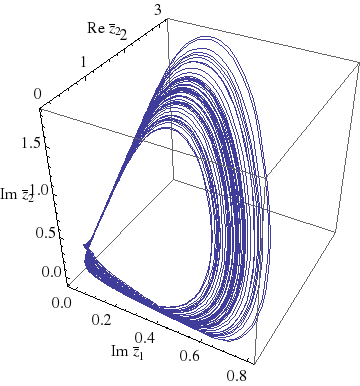
\includegraphics[width=0.6\textwidth]{2modesMFmixing.png}
%
% \caption{\twoMode\ dynamics in $(1,\,-1,\,1,\,1/2)$ slice}
%
% \label{fig:2modesMFmixing}
% \end{figure}
% %%%%%%%%%%%%%%%%%%%%%%%%%%%%%%%%%%%%%%%%%%%
%
% Note that there is some freedom in choosing the coefficients that lead to a slice mixing two specific modes.
%

% \item[2014-02-13 Evangelos] In general, if we would like to have a slice that
% couples modes $k$ and $j$, we have to choose $c_m'=b_m'=0$ for $m\neq k,j$
% and
% \begin{align}
%   k\, c_k' & =  - k^2\, b_k' = C_k \,,\label{eq:sliceMixing1}\\
%   j\, b_j' & =  j^2\, c_j'  =  C_j \,,\label{eq:sliceMixing2}
% \end{align}
% where $C_k=C_j\neq 0$ are constants. This would lead to chart border
% \beq\label{eq:ChartBordMixing}
%   c_k^* = b_j^* = 0\,.
% \eeq
% Alternatively, we may permute $k$ and $j$ in \refeqs{eq:sliceMixing1}{eq:sliceMixing2}
% to get chart border given by
% \beq
%    b_k^* = c_j^* = 0\,.
% \eeq
%
% Note that we are free to rotate the slice defined by \refeqs{eq:sliceMixing1}{eq:sliceMixing2}
% by any angle $\theta$.
%
% \item[2014-02-13 Evangelos] In the case of $\SOn{2}$ the dimension of
% the slice is $N=d-1$, where $d$ the dimension of the phase space.
% \refeq{eq:chartBordSlice} expresses the fact that the chart border must
% be on the slice. Then the constraint \refeq{eq:chartBord} implies that
% the chart border is a $d_b = N-1$ dimensional hyperplane. A trajectory
% on the slice has dimension $d_t=1$, and therefore $d_b+d_t=N$.
% By analogy to the case of a plane and a line in $3-D$, their
% intersection should be zero-dimensional, \ie, a  point, but we have
% to check this (in algebraic geometry books?). So far I do not get any
% great insight, except that we have some more freedom to choose slices
% with simple chart borders. In terms of dimension, all chart borders are
% created equal. But we might be able to pick slices with chart borders
% that physics does not like to visit.


\item[2014-02-12 Burak] I fixed a typo in my \KS\ python code and tried
integrating \refeq{eq:scaledtime} with 16 modes ($|a_0|=0$ and $L=22$)
using a standard integrator \texttt{scipy.integrate.odeint} (a wrapper
for \texttt{lsoda} from \texttt{odepack}) and actually got a chaotic looking
trajectory \reffig{fig:KSsspRedScaledTime}. When I tried the same integrator
on the full \statesp\ ODEs, it diverged, so the time scaling can actually
be easing the stiffness of the ODEs.\ES{maybe you could give us some details
or a plot to understand what the problem might be. Or is the plot
\reffig{fig:KSsspRedScaledTime}(b)? I do not see a divergence there.}

%%%%%%%%%%%%%%%%%%%%%%%%%%%%%%%%%%%%%%%%%%%
\begin{figure}%[H]
 \centering
 (a) 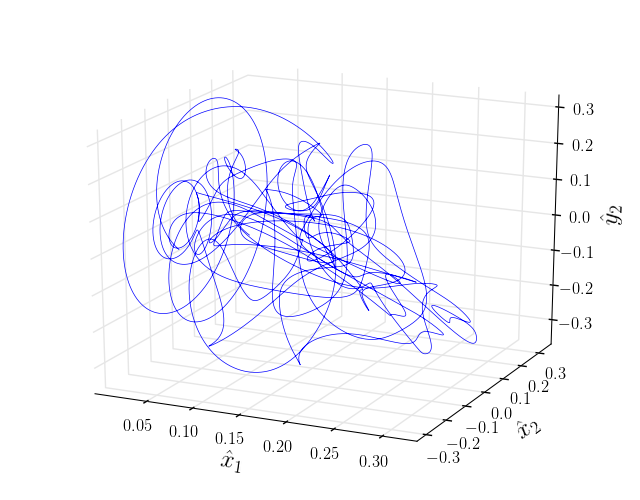
\includegraphics[width=0.45\textwidth]{KSsspRedScaledTime}
 (b) 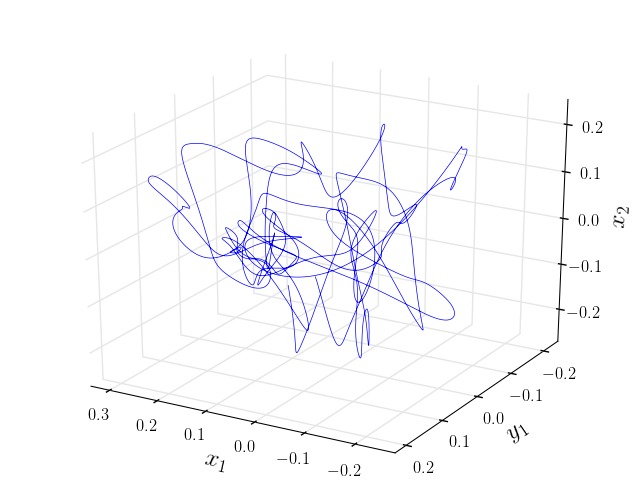
\includegraphics[width=0.45\textwidth]{KSsspReconst}
\caption{\KS\ dynamics integrated within the slice with a simple integrator
using scaled time formula \refeq{eq:scaledtime}: (a) in the \slicePlane\
(b) in the full \statesp.}
\label{fig:KSsspRedScaledTime}
\end{figure}
%%%%%%%%%%%%%%%%%%%%%%%%%%%%%%%%%%%%%%%%%%%

\refFig{fig:KSsspRedScaledTime} looks quiet different from the solution
I get from Ruslan's solver so it could be wrong. However, I don't actually
know how that solver (the one with forward/backward ffts) works, so may be
it's normal for two solutions to be completely different after Lyapunov time.
Any suggestion for checking the validity my solutions?

I thought, may be, I can try computing already known (relative) periodic
orbit trajectories. Do you have their data stored somewhere in this blog?

\item[2014-02-12 Evangelos] Ruslan's rpo's are in
\\
\texttt{siminos/matlab/ruslan/ks22f90h25t100.mat}.
I remember documenting the format in one of our blogs but I cannot find where.
The quickest way would be to ask Xiong Ding. He uses this database extensively.

I would suggest to try a short and not very unstable periodic orbit. Integrate it for $2T_p$ and
see if it closes back to itself.

\item[2014-02-12 Ruslan 2 Burak] You can read about it in
\\
\texttt{siminos/matlab/ruslan/00ReadMe.txt}.

\begin{figure}%[H]
 \centering
  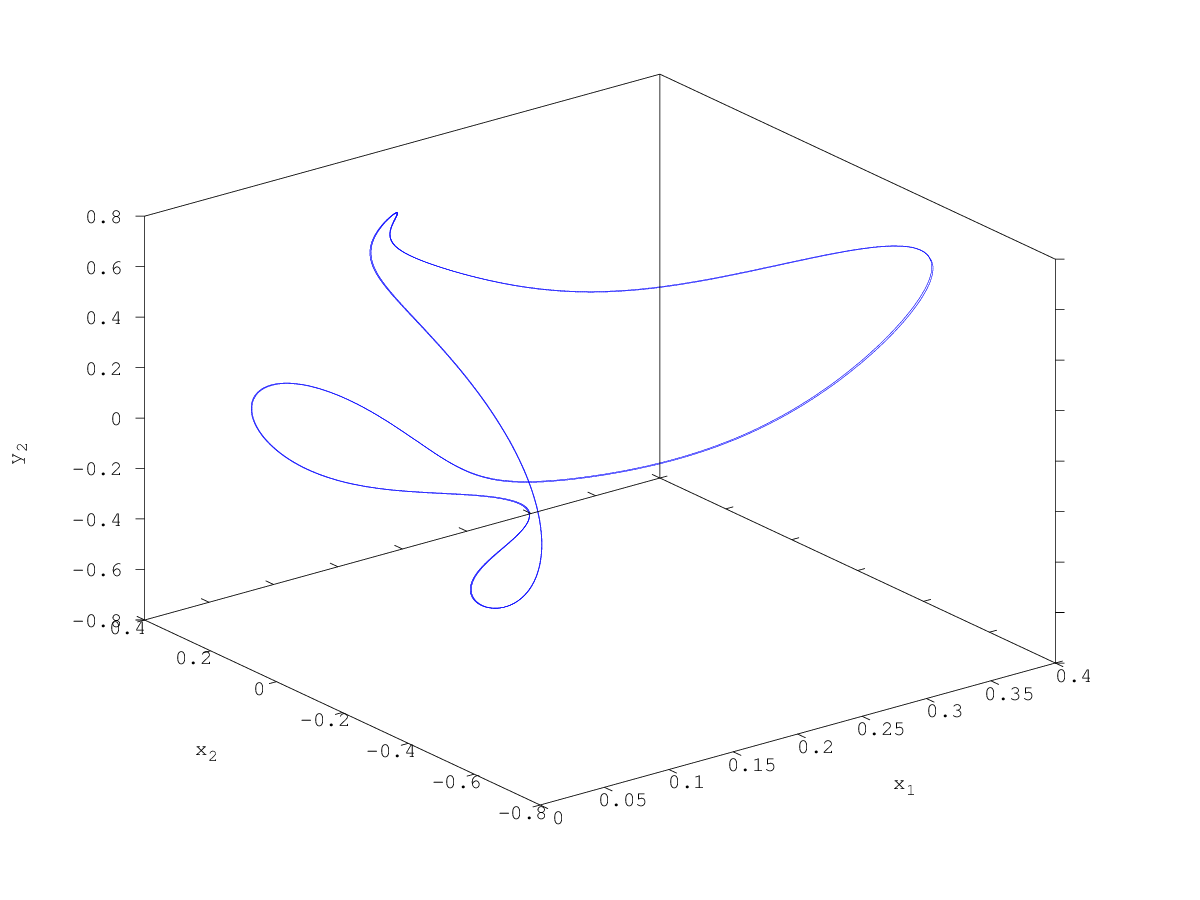
\includegraphics[width=0.6\textwidth]{ksslice_tscaled}
\caption{A \KS\ \rpo\ integrated within the first mode slice using scaled
	  time formula.}
\label{fig:ksslice_tscaled}
\end{figure}

\item[2014-02-13 Burak] I'm committing two short Matlab (tested only on Octave)
programs, both producing the same \reffig{fig:ksslice_tscaled} by
integrating \KS\ equation with the initial point corresponding to the first
\rpo\ in  \texttt{ks22f90h25t100.mat}. You can find the programs
\\
\texttt{ksETDRK4\_16mode\_L22\_hscaled.m } and
\\
\texttt{ksETDRK4\_16mode\_L22\_tscaled.m }
in
\\
\texttt{../budanur/KuramotoSivashinsky/}.
Both of them are adaptations of ETDRK4 of
\HREF{http://eprints.maths.ox.ac.uk/1194/1/NA-03-14.pdf}
{Kassam and Trefethen}\rf{ks05com}.
I'll explain the tweaks I did to make it work:

\renewcommand{\ssp}{a}             % state space point
\renewcommand{\pSRed}{\ensuremath{\hat{\cal M}}} % reduced state space
\renewcommand{\sspRed}{\ensuremath{\hat{\ssp}}}    % reduced state space point, experiment
\renewcommand{\velRed}{\ensuremath{\hat{\vel}}}    % ES reduced state space velocity
\renewcommand{\slicep}{\ensuremath{\hat{\ssp}'}}   % slice-fixing point, experimental

I started with deriving the scaled time formula for \Un{1}, which is the continuous
symmetry group if we represent the problem in terms of $M$ complex Fourier modes.
Lie algebra generator of $\Un{1}$ is diagonal:
    \PC{2014-02-14 to get to modes $0, 1, ..., M$, rather than $k \in
    [-M, \cdots, M]$ you already used the reality of $u(x,\zeit)$, right?
    Also $k=0$ is not there by Galilean invariance. Presumably already
    built into ETDRK4...}
\beq \label{eq:LgU1}
   \Lg_{ij} = i\,\delta_{ij} \,,\qquad i,j = 0, 1, ..., M.
\eeq
In this representation, the first mode template is written as:
\beq \label{eq:slicepU1}
    \slicep = (1+0\,i, 0, 0, 0, ..., 0)
\eeq
Using these definitions, we can write the \refeq{eq:so2reduced} explicitly as:
\bea
\velRed(\sspRed) &=& \vel(\sspRed)
   -\frac{\Im[\vel(\sspRed)_1]}{\Re[\sspRed_1]} \, \groupTan(\sspRed)
\continue
\dot{\gSpace}(\sspRed) &=& \frac{\Im[\vel(\sspRed)_1]}{\Re[\sspRed_1]}
\,.
\label{eq:u1reduced}
\eea
Note the extra minus sign. Now to be able to use ETDRK4 to integrate these,
we have to split this velocity function to its linear and non-linear parts.
\KS\ equation in Fourier domain can be written as:
\beq\label{eq:KSLN}
  \vel (\ssp) = L \ssp + N(\ssp)
\eeq
Here $L_k = q_k^2 - q_k^4$ is the linear (diagonal in Fourier domain), whereas
$N(x)$ is the nonlinear, discrete convolution term. We can write the reduced
velocity function \refeq{eq:u1reduced} in the same form,
\beq\label{eq:LhatNhat}
  \hat{L} = L
  \,,\qquad
  \hat{N}(\sspRed)  = N(\ssp)
  -\frac{\Im[\vel(\sspRed)_1]}{\Re[\sspRed_1]} \, \groupTan(\sspRed) .
\eeq
and apply the ETDRK4 algorithm to $\velRed(\sspRed) = \hat{L} \sspRed + \hat{N}(\sspRed) $.
In order to have a control on the near-singularity behavior of the \refeq{eq:u1reduced},
I scaled the time step $h$ in every iteration using the following rule:
\beq
  h = \left\{
	\begin{array}{ll}
		|\Re[\sspRed_1] | h_0  	& \mbox{if } |\Re[\sspRed_1] |  < 1 \\
		 h_0		        & \mbox{otherwise }
	\end{array}
\right.
\eeq
This is how \texttt{ksETDRK4\_16mode\_L22\_hscaled.m} works. The price
we pay here is, we have to re-compute the ``exponential means" of the ETDRK4
algorithm every time we use a time step different than $h_0$. We can get rid
off this by defining $d \tau = \Re[\sspRed_1]^{-1} dt$ and writing
\refeq{eq:u1reduced} in terms of the scaled time:
\bea
 \frac{d \sspRed}{d \tau}  &=& \Re[\sspRed_1] \vel(\sspRed)
	- \Im[\vel(\sspRed)_1] \, \groupTan(\sspRed)
\continue
\frac{d \gSpace}{d \tau} &=& \Im[\vel(\sspRed)_1]
\,.
\label{eq:u1scaled}
\eea
Final trick is to get \refeq{eq:u1scaled} into the same form with \refeq{eq:KSLN}.
To do this, we add and subtract $1$ to the $\Re[\sspRed_1]$ in the first line of
\refeq{eq:u1scaled} and define:
\bea\label{eq:LtildeNtilde}
  \tilde{L} &=& L ,
  \continue
  \tilde{N}(\sspRed) &=& N(\sspRed) + (\Re[\sspRed_1] - 1) \vel (\sspRed)
  			- \Im[\vel(\sspRed)_1] \, \groupTan(\sspRed) .
\eea
Using these definitions, we can now apply ETDRK4 scheme to integrate
\beq\label{eq:}
  \frac{d \sspRed}{d \tau} = \tilde{L} \sspRed + \tilde{N}(\sspRed) .
\eeq
\ES{I am bit confused here. You seem to have a stiff term in your $\tilde{N}$, since
\vel (\sspRed) contains $L$. Then using ETDRK4 would not help you with stiffness.
{\bf Burak:} You are right. I don't have a rigorous justification for why
this works, I just tried a few different things. One thing that may be an
explanation is that the term that contains $L$  in $\tilde{N}$ in \refeq{eq:LtildeNtilde}
has its sign flipped: $(Re[\sspRed_1] - 1 < 0)$ (by just looking at plots)
all the time, so its effect should be slowing down the modes. If this is
what makes this adaptation work, may be we could do the add/subtract trick
with a tunable parameter rather than $1$ and make sure that the stiff term
that is transferred to the nonlinear part always has its sign flipped so
that the ETDRK4 can work. {\bf Evangelos:} I don't think the sign matters
when you have stiff terms. What time step are you using for this integration?
Maybe you end up using smaller time step than what you would use with ETDRK4?
{\bf Burak:} $h = 0.1$ for the scaled time steps.
}
This is how \texttt{ksETDRK4\_16mode\_L22\_tscaled.m} works. Both methods
produce \reffig{fig:ksslice_tscaled} in less than $20$ seconds on my laptop.

\item[2014-02-24 Evangelos] Both scaled time equations
\refeq{eq:scaledtime} and \refeq{eq:scaledtimeGeneral}
have a fixed point at the chart border (note that the second term
merely keeps integration on the slice, while the first term vanishes
at the chart border). This is OK as long as the the trajectory
one integrates does not hit the chart border, but would mean that one
has to switch slice, if the chart border is reached in finite time.
Since the argument that trajectories do not hit the first fourier mode slice
is probabilistic, maybe it would be interesting for Burak to plot a
time series of $x_1$ for the turbulent trajectory of KS he uses in his
simulations. A slice crossing would correspond to stagnation at $x_1=0$.

\item[2014-02-24 Burak] I think this is a valuable observation. To have a
more precise argument about safety of a particular single-mode \slice\ we
should look at the eigenvalues and eigenvectors of the stability matrix,
we can than search for the stable/unstable manifolds of this fixed point
and move forward beyond the probabilistic argument. My guess is that chart
border will be a set of unstable equilibra for \KSe\ and we will have physical
interpretations for stable/unstable manifolds as stable/unstable manifolds
of equilibria in the 2nd and 3rd mode invariant subspace.

\item[2014-02-24 Evangelos 2 Burak] This is an interesting line of thought, you should
definitely follow through with it! I think you can safely let the second term aside (it corresponds
to dynamics transverse to the slice) and concentrate
on $|\braket{\groupTan(\sspRed)}{\sliceTan{}}|\, \vel(\sspRed)$
(but don't take my word for it, at the end you should check if this is sufficient).

Then, it's all quite simple for the first Fourier mode slice. The stability matrix reads
\beq
  A_{ij} = \frac{\partial \tilde{v}_i}{\partial x_j} = \delta_{11}\, v_i + x_1 \frac{\partial v_i}{\partial x_j}
\eeq
and for $x_1=y_1=0$, it takes the particularly simple form
\beq
  A_{ij} = \frac{\partial v_i}{\partial x_j} = \delta_{11}\, \left. v_1\right|_{x_1=y_1=0}
\eeq
The sign of the eigenvalue depends on the sign of the velocity field of the real part of the first fourier mode.
You might be able to infer something by having a look at the nonlinear terms of KS in fourier space
(please first check for mistakes in what I have written, as usual).

\item[2014-02-24 Burak] Scaled time equations does not have a fixed point
at $\hat{b}_1 = 0$, but, it's an invariant subspace. First term in \refeq{eq:scaledtime}
vanishes because it is multiplied by $\hat{b}_1$, and in the second term, we
have $\Lg \hat{x} = (0, 0, 2 y_2, -2 x_2, 3 y_3, -3 y_3, ...)$ so what happens
in $\hat{b}_1 = 0$ stays in $\hat{b}_1 = 0$. This pactually roves that \refeq{eq:scaledtime}
is totally safe to integrate. Note that, this actually is cheating, this
happens as a result of our particular redefinition of time. However, the
solutions so far we got from this approach are accurete and smooth, and there
seems to be no reason for them to be otherwise.

\item[2014-02-26 Evangelos 2 Burak] Actually, scaled equations do have fixed points
at $\hat{b}_1 = 0$. You forget that the second term also
contains $\braket{\vel(\sspRed)}{\sliceTan{}}$, which kills all velocity components
for Fourier modes higher than one. Combined with the $\Lg \hat{x}$ contribution which
kills the first Fourier mode velocity component, you get a fixed point at the chart
border. This is consistent with the role that the second term plays (it subtracts
velocity contribution transverse to the slice).

\item[2014-02-26 Burak 2 Evangelos] I think you confused yourself just like\HREF{https://piazza.com/class/hqlfc5pslb5nv?cid=47}{this}
anonymous (see the follow up discussion) student in Chaosbook class.

\item[2014-02-26 Burak] In general, what happens with scaled time equations
is that, if your real trajectory tends to go to $x_1 = 0$ it would take infinitely
long time to arrive there by integrating \refeq{eq:scaledtime}. This doesn't
mean that there is something wrong or artificial with the description, in fact,
it just shows that the method is robust. You would never get a wrong solution
from it, in fact, you'd know when it's time to go to another slice if you
have a weird system that frequently visits $a_1 = 0$.

\item[2014-02-26 Evangelos] There is no confusion, and probably no disagreement here.
\refeq{eq:scaledtime} is a dynamical system in its own right, and it has fixed points
that sit on the chart border. In any dynamical system, attracting fixed points can only
be reached in infinite time by a trajectory along their stable manifold,
so we are cool here. What is interesting here, is that you can use this property to tell
you that you have to switch slice.

\item[2014-02-26 Evangelos] Added figure to illustrate that when we hit the chart border
in rescaled time integration, we actually approach a stagnation point. For the slice defined by
$(1,-1,1, 1/2)$, the chart border is hit by a chaotic trajectory. Once this happens we cannot integrate
past the chart border, and we would have to switch slice. Note that $|\braket{\groupTan(\sspRed)}{\sliceTan{}}|$,
which is a measure of distance from chart border, quickly reaches machine epsilon.

On the other hand, for slice defined by $(1,0,0,0)$, the chart border is an invariant subspace
and although integration slows down at close passages to it, the distance from the chart border
remains bounded away from zero.

Burak, I think it would be interesting to replicate the plots (b)/(d) for KS with the first mode slice.
It becomes very clear whether you hit the chart border or not.

Here, a variable step size integrator is used, but I don't think using a fixed step size integr2tor would
affect the results.

\begin{figure}%[ht]
\begin{center}
(a)~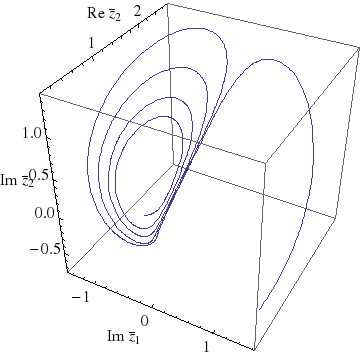
\includegraphics[width=0.35\textwidth]{2modesSliceInt_hit.png}~
(b)~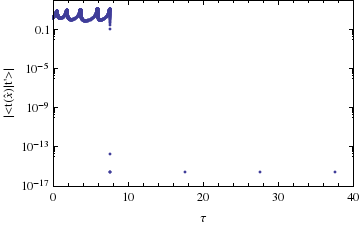
\includegraphics[width=0.50\textwidth]{2modesChartBordCond_hit.png}\\
(c)~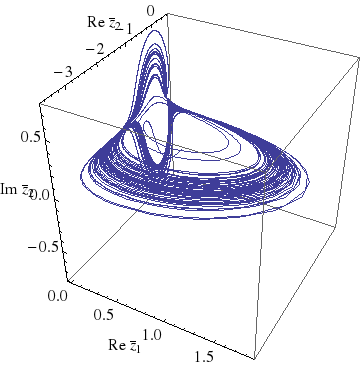
\includegraphics[width=0.35\textwidth]{2modesSliceInt_miss.png}~
(d)~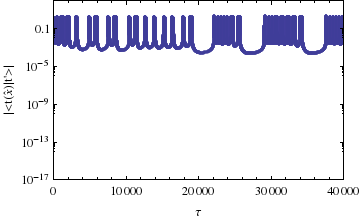
\includegraphics[width=0.50\textwidth]{2modesChartBordCond_miss.png}\\
(e)~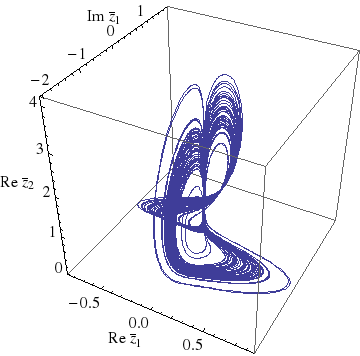
\includegraphics[width=0.35\textwidth]{2modesSliceInt_2f.png}~
(f)~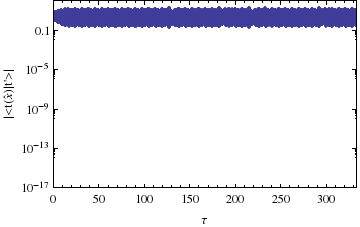
\includegraphics[width=0.50\textwidth]{2modesChartBordCond_2f.png}
\end{center}
\caption{(a) Two-modes system integrated on the $(1,-1,1, 1/2)$ slice. (b)$|\langle\groupTan(\sspRed)|\sliceTan{}\rangle|$
as a measure of distance from chart border on points along the same trajectory.
Note that a variable step size integrator is used, which takes large steps once an equilibrium is approached.
(c) Two-modes system integrated on the $(1,0,0,0)$ slice.
(d) $|\langle\groupTan(\sspRed)|\sliceTan{}\rangle|$ along the same trajectory.
(e) Two-modes system integrated on the $(0,0,1,0)$ slice.
(f) $|\langle\groupTan(\sspRed)|\sliceTan{}\rangle|$ along the same trajectory.
    }
\label{fig:2modes_hit}
\end{figure}

\item[2014-02-24 Evangelos] Actually there is more grace in
checking if the integrator has hit a fixed point, rather than having to
deal with discontinuous jumps, in order to change slice, if one decides
to work with general slices.

\item[2014-02-24 Burak] I started this whole thing by first checking whether
the first Fourier mode amplitude vanishes for a typical \KSe\ solution, and
my observation was it gets close but never actually become exactly 0.

\item[2014-02-24 Evangelos] In finite precision arithmetic, it would be very hard
to get exactly $a_1=0$. But in rescaled time, you could get to this fixed point,
if it is attractive. So I think it is worth rechecking for the rescaled time
integration on the slice.

\item[2014-02-24 Evangelos] To illustrate why I am still a bit unhappy
with first mode slice, I copy from my thesis the explicit form of the transformations
implied by fixing the first fourier mode (define slice by $c_1=Im(a_1)=0$):
\beq\label{tab:SO2n6}
\scriptsize
\begin{array}{ll}
  u_1=r_1=\sqrt{b_1^2+c_1^2}&  \\ u_3=\frac{b_2 \left(b_1^2-c_1^2\right)+2 b_1 c_1 c_2}{r_1^2}&u_4=\frac{-2
b_1 b_2 c_1+\left(b_1^2-c_1^2\right) c_2}{r_1^2}\\ u_5=\frac{b_1 b_3 \left(b_1^2-3 c_1^2\right)-c_1 \left(-3
b_1^2+c_1^2\right) c_3}{r_1^3}&u_6=\frac{-3 b_1^2 b_3 c_1+b_3 c_1^3+b_1^3 c_3-3 b_1 c_1^2 c_3}{r_1^3}\\ u_7=\frac{b_4
\left(b_1^4-6 b_1^2 c_1^2+c_1^4\right)+4 b_1 c_1 \left(b_1^2-c_1^2\right) c_4}{r_1^4}&u_8=\frac{4 b_1
b_4 c_1 \left(-b_1^2+c_1^2\right)+\left(b_1^4-6 b_1^2 c_1^2+c_1^4\right) c_4}{r_1^4}\\ u_9=\frac{b_1
b_5 \left(b_1^4-10 b_1^2 c_1^2+5 c_1^4\right)+c_1 \left(5 b_1^4-10 b_1^2 c_1^2+c_1^4\right) c_5}{r_1^5}&u_{10}=\frac{-b_5
c_1 \left(5 b_1^4-10 b_1^2 c_1^2+c_1^4\right)+b_1 \left(b_1^4-10 b_1^2 c_1^2+5 c_1^4\right) c_5}{r_1^5}\\ u_{11}=\frac{b_6
\left(b_1^6-15 b_1^4 c_1^2+15 b_1^2 c_1^4-c_1^6\right)+2 b_1 c_1 \left(3 b_1^4-10 b_1^2 c_1^2+3 c_1^4\right) c_6}{r_1^6}&u_{12}=\frac{-2
b_1 b_6 c_1 \left(3 b_1^4-10 b_1^2 c_1^2+3 c_1^4\right)+\left(b_1^6-15 b_1^4 c_1^2+15 b_1^2 c_1^4-c_1^6\right) c_6}{r_1^6}\\
\end{array}
\eeq
\normalsize

I got these using mathematica, but you can derive the first few by hand by a
few trigonometric transformations.

The problem with first mode slice becomes apparent when you try to think how the 2- and 3- mode
equilibria $E_2$ and $E_3$ are represented in these variables. Both of them have $a_1=0$
and therefore lie on the chart border (actually, you do not need the explicit expressions
\refeq{tab:SO2n6} in order to come to this conclusion).
Moreover, both $E_2$ and $E_3$ are dynamically important,
so we cannot say ``who cares''. Many of the rpo's visit them, and the real challenge is to put
those on the slice in a manner that allows to understand their dynamics. My hint here would be
to try to use the unstable manifolds of $E_2$ and $E_3$ which will probably not lie on the
chart border.

If you insist on using a single slice, I would think that the second or third fourier mode would be even more
natural for KS. Moreover, it might be even better to use the sixth fourier mode ($E_2$ has vanishing
third mode, while $E_3$ has vanishing second mode. Both $E_2$ and $E_3$ have non-vanishing sixth mode).
By the same probabilistic argument as for the first Fourier mode, you should not hit the slice border.

\item[2014-02-24 Burak] 2nd-mode harmonics and 3rd-mode harmonics are invariant
subspaces of the \KS . We discussed this before and my suggestion was to apply
the first mode recipe as if the 2nd or 3rd mode is the first mode for their
respective invariant subspaces. 6th mode is also worth to experiment with,
but as I said, I did not simply ignore 2nd and 3rd mode invariant subspaces.

\item[2014-02-24 Evangelos 2 Burak] I do not understand the flow-invariant subspace argument, could you
please explain/sketch the derivation?

\item[2014-02-24 Burak] Since the second mode and its harmonics form an
invariant subspace, trajectories starting in this invariant subspace will
stay in it. Now you can redefine the system size from $L$ to $L/2$ for \KS ,
and your symmetric boundary conditions would still be satisfied for the
system size being $L/2$ since all your modes are harmonics of the 2nd. In
this representation, what previously was the 2nd Fourier mode is the 1st
mode, 4th is the 2nd and so on... Same argument can be made for the 3rd mode
harmonics and any invariant subspace formed by the harmonics of a prime mode.
This probably is true for any flow with nonlinear terms to the 2nd order,
you can see why harmonics of the prime numbers form invariant subspaces by
writing the convolution term in the \KSe\ explicitly. By doing so, you will
get a term like $\sum_{k,l} e^{i (k+l) x}$ and if both $k$ and $l$ are multiples
of a prime number, then so is their sum, thus you can't generate any mode
outside the invariant subspace.

\item[2014-02-28 Predrag] ``Harmonic" seems a fancy word, I gave
ChaosBook.org ver. 14.5.*
{\em Example 10.4 Invariance under fractional rotations} as an exercise
to Xiong Ding and Burak to explain why $\Zn{m}$ subgroups of $\SOn{2}$
are flow-invariant subspaces; they are just $m$-copies tailings of the full
space by a periodic B.C.
fundamental domain. $m$ is any integer (nothing special about primes, I believe).
Unfortunately, these subspaces do not fill up the entire \chartBord\ - as you observe,
a generic initial condition within the single-Fourier mode slice flows out
into the big world.
If you have a suggestion how to make this clearer, let me know.


\item[2014-02-25 Xiong to Burak] I am sorry I still cannot
understand the reasoning about the invariant subspaces spanned by
harmonics of prime numbers.

The nonlinear term of velocity field is
$-i\dfrac{q_k}{2}F_{n}[(F_N^{-1}[a])^2]_k$. I agree with you that
the product of back Fourier transforms $(F_N^{-1}[a])^2$ will
generate $\sum_{k,l} e^{i (k+l) x}$, but the Fourier transform
$F_{n}[]_k$ will mix all modes. It is not simply summed, it is weighted
by $e^{iq_{k}x_{n}}$. The backward and forward Fourier
transform is the standard way to deal with nonlinear terms in spectral
method, which is different from finite difference method that the
derivative at each point is non-local. The expansion of the convolution is
$\sum_{m=-\infty}^{+\infty}a_{m}a_{k-m}$. Probably I am wrong.

\item[2014-02-25 Burak to Xiong] If you agree that the terms you get are
in $a_k a_l e^{i (k+l) x}$ form then you should be convinced because Fourier
transform cannot mix modes. Note:
\beq
 \int_0^L dx e^{i (k+l) x} e^{- i n x} = 2 \pi \delta_{k+l,n}
\eeq

\item[2014-02-26 Evangelos to Burak and Xiong] I agree with Xiong.
I derived explicit expressions for the velocity field of KS written in terms
of real and imaginary parts for my thesis (see Eqs. 115-116 in the online version
on chaosbook.org). Unless I am wrong, there is contribution from
the nonlinear terms that brings you outside these ``harmonic subspaces.''

Anyway, I do not see why this argument would prevent you to use second or third
Fourier mode slice. It's easy to implement, just do it!


\item[2014-02-26 Burak to Evangelos] I'm sorry to say this but you cannot
just disagree with my argument while it has equations and delta functions
in it. I can only say that by writing convolutions explicitely you probably
hid some cancellations and got the wrong impression that modes generate
subharmonics. I also remember that in one of your papers or thesis you
mentioned $n=2,4,6,...$ and $n=3,6,,9,...$ are invariant subspaces.

I also never mentioned that you cannot use 2nd or 3rd mode because they are
part of invariant subspaces; I only told you that I don't ignore $2nd$ and
$3rd$ mode harmonics invariant subspaces and tried to explain how I plan
deal with them.

\item[2014-02-26 Evangelos to Burak] But Burak, if you don't write this clearly,
we will not understand it. You have one Kronecker delta and a double sum,
so what I can see from what you write is that the convolution term is still
$\sum_{m=-\infty}^{+\infty}a_{m}a_{k-m}$. This does not help me see why
your claim is true. Or I got it all wrong, and I do not follow you at all?

Now, thanks for reminding me about the fixed point subspaces of $\On{2}$.
I think this is what you saw in my thesis, and indeed these are invariant
subspaces of KS flow (or any flow with \On{2} symmetry), by a well known
theorem. I now find my thesis very hard to read, but I think you are correct that these are
subspaces which correspond to harmonics of a basic $k$ (however I do not see
why you say that this $k$ has to be prime).

Of course, apart from the group theoretic way to get these
subspaces, there should be a direct way to see them in the velocity field,
but I still cannot see how your Kronecker delta leads to that.

Anyway, this is not an important point to get stuck to. The important thing,
on which I hope we are on the same page, is that if you use, e.g., second mode slice,
you will not work with a system that has $a_1=0$ and you should not redefine your
box size. You will just use the slice $(0,0,1,0,\ldots)$,
for a generic trajectory. You are allowed to do that, and I think you should
not face any difficulties.

\item[2014-02-25 Xiong to Ruslan] If points are group transformed
onto the slice after evolving the system in the full state space,
could I find a simple way to transform the Jacobian matrix too
(make it one dimension less), or the covariant vectors?

\item[2014-02-28 Predrag to Xiong Ding] This has been a
ChaosBook.org homework for you and Kimberly since September,  so why don't you just do it and write it up? For {\jacobianMs} argument is along the lines we
used for the
\HREF{http://www.streamsound.dk/book1/chaos/chaos.html\#126/z}
{\PoincSec s} (possibly simpler) and
for eigenvectors I sketched it out for you on a blackboard yesterday, so
please write it up someplace in your blog...



\renewcommand{\ssp}{a}

\item[2014-02-14 Burak] I discovered an Octave / Matlab incompatibility in
my mfiles that is so \HREF{http://matlabsadness.tumblr.com/post/46623593831/non-orthogonal-indexing}{Matlab's fault}
that I don't want to correct it. It will kill the code's readability if I
do so. My next plan is to call octave from python anyways, so I'm not touching
those files right now. If you want to play with them, here is how you do
it on a unix machine with an Octave installation:

\texttt{octave --persist ksETDRK4\_16mode\_L22\_tscaled.m}


\end{description}

\section{Burak's daily blog}
\label{sect-dailyBlogBB}

\begin{description}

\item[2013-11-15  Predrag] Brought Burak's blog from \texttt{gitHub} exile back to Evangelical home, so I do not have to copy stuff back and forth. The draft of the magic slice article still remains in the  \texttt{gitHub} exile \texttt{reducesymm/cgang/}. We have to respect Divakar's edicts.

\item[2013-07-11  Predrag to Burak] The last common entry with the svn repository
\\
\texttt{siminos/blog/dailyBlog.tex} is

{\bf [2013-03-14 Evangelos]} In
\emph{Quasiperiodic oscillations and homoclinic orbits in the nonlinear nonlocal
Schr\"odinger equation}, \arXiv{1303.3213}...

then the two blogs diverge. This file
\texttt{reducesymm/blog/dailyBlogBB.tex}
has only Burak work; do not edit anything in
the older \texttt{reducesymm/blog/dailyBlog.tex}

\item[2013-07-07  Predrag]
Burak (Nazmi B. Budanur <burakbudanur@gmail.com>), a new theory graduate student, started at GaTech Aug 2013, is joining us. He will focus on slicing, hopefully
slicing for pipe flows.

\item[2013-07-11  Predrag to Burak]
A better version of today's tutorial:
\HREF{http://chaosbook.org/~predrag/papers/WHole12.pdf} {8 Aug 2012 talk}.

Read \HREF{http://www.cns.gatech.edu/~predrag/papers/preprints.html\#atlas12} {Cvitanovi\'c \etal} \emph{Cartography of high-dimensional flows: A visual guide to sections and slices}\rf{atlas12}, blog here about things you understand or do not understand.

\item[2013-07-12  Burak] I started feeling lost in section IV of the
    paper. I think I should work on simpler examples of \PoincSec s
    and method of slices to make the distinction well. For
    that purpose, I thought about going through examples of Chapter III
    of ChaosBook and then trying to reproduce
    \HREF{http://www.cns.gatech.edu/~predrag/papers/FrCv11.pdf}
    {Froehlich \& Cvitanovi\'c} \emph{Reduction of continuous
    symmetries of chaotic flows by the method of slices}\rf{FrCv11}. Is
    this a good idea?

\item[2013-07-12  Predrag] I would go through
\wwwcb{/paper.shtml\#maps} {\em Chapter  - Discrete time dynamics} examples first, then
we think of the next step?

\item[2013-07-12  Burak]
I did not get an e-mail notification after your commit yesterday and I found out that it is not default in github.

To get notifications for commits, under
\begin{verbatim}
Settings -> Service Hooks -> E-mail
\end{verbatim}
You should enter e-mails that we want the notifications to be sent.

I checked this on one of my repository and it works.

What is annoying is, we can only enter two e-mail addresses in this area, which is not a problem right now but it will be when others join github. To work this around, I can set up a ``forwarder" e-mail address for the project which would forward the e-mails that it receives to the participants of the project so that everyone can be notified.
\item[2013-07-12  Predrag] Check whether paid accounts have unlimited email lists (I seem to remember that bitBucket free accounts were up to 5 collaborators). I
    do not mind paying from a grant, if the thing works...

\item[2013-07-15  Burak]
I talked to the github support and learned that they do not send notifications for pushes. I then checked Bitbucket (github clone), setting up e-mail notifications is pretty similar:
\begin{verbatim}
Settings -> Services -> E-mail->Add service
\end{verbatim}
As you said, we are also able to get private repositories with up to 5 collaborators on Bitbucket.

It is also possible to workaround this problem on github by starting a mail list and setting that up such that it forwards mails it recieves from github to the people on the list.

\item[2013-07-15  Burak]
I have done most of the exercises 2.8, 3.1, 3.2, 3.7 (ChaosBook
version14.4.1) and re-read the paper.

In exercise 3.2 what exactly do you mean by ``Euclidean length s
computed curvilinearly along the attractor section''? Is it the
distance along the orbit?
\item[2013-07-18  Predrag] Read
Section 12.1.1 {\em Parametrization of invariant manifolds}. I've now
included link to this section in exercise 3.2 {\em A return Poincar\'e
map for the R\"ossler flow.}

\item[2013-07-15  Burak]
Another question about
\HREF{http://www.cns.gatech.edu/~predrag/papers/preprints.html\#atlas12}
{Cvitanovi\'c \etal} \emph{Cartography of high-dimensional flows: A
visual guide to sections and slices}\rf{atlas12}. How do you get the
tangent vector in the extremum condition, eqs.~(6), (7). I would
understand it if the transformation was infinitesimal but I do not see
it for $\gSpace$ from 0 to $2 \pi$.
\item[2013-07-18  Predrag]
We discussed it today - can you write down the answer here?

\item[2013-07-21  Burak] In the equation, $\sspRed$ is $\ssp$,
    transformed like $\sspRed = \LieEl^{-1}(\gSpace) \ssp$ such that it is closest
    to the template point $\slicep$. Now, it does geometrically make
    sense to me that the extremum condition should require that vectors
    $(\sspRed - \slicep)$ and $ \sliceTan{} = \Lg \slicep$ to be
    perpendicular to each other, however, I still am not able to show
    this algebraically by just taking the derivative with respect to
    $\gSpace$.
\item[2013-07-22  Predrag] Bummer, read
    \HREF{http://chaosbook.org/paper.shtml\#continuous} {Chapter 10} -
    {\em Relativity for cyclists} very critically, I have to rewrite
discussion of slicing (still have not described the extremal distance
condition). Please reread the argument in Froehlich \&
Cvitanovi\'c\rf{FrCv11}, if it now makes sense to you, summarize the
argument here, with an eye on having me update this in ChaosBook...

\item[2013-07-15  Burak] Going through
    \HREF{http://chaosbook.org/paper.shtml\#maps} {Chapter 3} and
    examples was really helpful, should I continue with
    \HREF{http://chaosbook.org/paper.shtml\#continuous} {Chapter 10} -
    {\em Relativity for cyclists} \&
    \HREF{http://chaosbook.org/paper.shtml\#knead} {Chapter 11} -
    {\em Charting the state space?}
\item[2013-07-18  Predrag]
We discussed it today - enter the plan here?

\item[2013-07-21  Burak] The current plan is, before Chapter 10, I will
    finish  \HREF{http://chaosbook.org/paper.shtml\#discrete} {Chapter
    9} - {\em World in a mirror} and after going through Chapter 10 and
    11, I will have a look at the Porter-Knobloch blog and try to find
    parameters that can make the equations behave chaotic.

\item[2013-07-23  Burak] Question on the derivation of eq. (10.51) of \HREF{http://chaosbook.org/paper.shtml\#continuous} {Chapter 10} - {\em Relativity for cyclists}: We have the slice condition:
\beq
 \sspRed^T \sliceTan{a} = 0.
\eeq
Substituting (10.49), I would have written down its time derivative as
\beq
 \velRed^T \sliceTan{a} = v(\sspRed)^T \sliceTan{a} - \dot{\phi}(\sspRed) \cdot t(\sspRed)^T \sliceTan{a}=0.
\eeq
However, this, in ChaosBook, is written as
\beq
 \velRed^T \sliceTan{a} = v(\sspRed)^T \sliceTan{a} - \dot{\phi_a}(\sspRed) \cdot t(\sspRed)^T \sliceTan{a}=0.
\eeq
I thought, $\phi \cdot \groupTan$ meant $\phi_1 t_1 + \phi_2 t_2 + \phi_3 t_3 + ... $ is this accurate? If so, dot product of a particular $\phi_a$ with $t(\sspRed)^T$ doesn't make sense to me. You also drop the indice a from the template tangent vector on the denominator of 10.51 and write it as dot product of tangent at x and the template tangent. I cannot see this
as well.

\item[2013-07-24  Predrag]
You poked your finger into a painful spot - We have used the
slicing condition only on Abelian cases such as $\SOn{2}$ and
$\SOn{2}\times\SOn{2}$, and I had never derived the correct formula for
non-Abelian case.

See
{\bf [2011-07-08 PC]} above (currently p.~89)
{\bf [2011-07-08 Predrag]} above (currently p.~115).
Someplace (in Froehlich?) we say that we would have to invert a matrix in
the general case - anyway, my formula is probably wrong, try to do it
your own way. Git pushing all figures for atlas12.tex paper now, might
continue on this later.

\item[2013-07-25  Predrag] (continued). Here is what we write in
\refref{FrCv11}, Sect.~{\em Dynamics within a slice}:
%\label{sec:mslices}

Any \statesp\ trajectory can be written in a factorized
form $\ssp(\tau)=\LieEl(\tau)\,\sspRed(\tau)$
(here $\LieEl(\tau)$ is a shorthand for $\LieEl(\gSpace(\tau))$,
or perhaps even $\LieEl(\gSpace(\ssp(\tau)))$).
Differentiating both sides with respect to time and
setting $\velRed={d\sspRed}/{d\tau}$ we find
\(
\vel(\ssp)=\dot{\LieEl} \, \sspRed+\LieEl \, \velRed(\sspRed)
\,.
\)
By the equivariance %\refeq{eq:FiniteRot}
\[
\vel(\sspRed)=\velRed(\sspRed) + \LieEl^{-1} \, \dot{\LieEl} \, \sspRed
\,.
\]
Noting that $\LieEl^{-1}\dot{\LieEl}=e^{-\gSpace \cdot \Lg} \,
\frac{d ~~}{d \, \tau} e^{\gSpace \cdot \Lg}=\dot{\gSpace}\cdot \Lg$,
we obtain the equation for the velocity of the reduced flow:
\beq
\velRed(\sspRed)=\vel(\sspRed)-\dot{\gSpace}(\sspRed)\cdot \groupTan(\sspRed)
\,.
\ee{eq:redVel}
The velocity $\vel$ in the full \statesp\ is thus the sum of the
`phase' velocity %\refeq{PC:groupTan1}
along the group orbit, $\dot{\gSpace} \cdot \groupTan(\sspRed)$,
and the remainder $\velRed$.

Eq. \refeq{eq:redVel} is true for any factorization
$\ssp=\LieEl \sspRed$, and by itself provides no
information on how to calculate $\dot{\gSpace}$. That is attained by
demanding that the reduced trajectory stays within a slice, by imposing
the slice conditions: % \refeq{PCsectQ}:
% PC 2013-07-25 added 2. equation
\bea
       \braket{\dot{\gSpace}\cdot \groupTan(\sspRed)}{\sliceTan{a}}
 &=& \braket{\vel(\sspRed)}{\sliceTan{a}}
    \continue
\sum_b \dot{\gSpace}_b \braket{ \groupTan{}_b(\sspRed)}{\sliceTan{a}}
 &=&
\braket{\vel(\sspRed)}{\sliceTan{a}}
\,.
\label{eq:slicecondition}
\eea
This is a matrix equation for the $N$\dmn\ vector $\dot{\gSpace}_b$ solved
by inverting the \statesp\ position dependent matrix
$\braket{\groupTan_b(\sspRed)}{\sliceTan{a}}$.
We consider here only the
$\SOn{2}$ case, which has a single group tangent:
\bea
\velRed(\sspRed) &=& \vel(\sspRed)
   -\dot{\gSpace}(\sspRed) \, \groupTan(\sspRed)
\continue
\dot{\gSpace}(\sspRed) &=& {\braket{\vel(\sspRed)}{\sliceTan{}}}/
               {\braket{\groupTan(\sspRed)}{\sliceTan{}}}
\,.
\label{eq:so2reduced1}
\eea
One way to think about this reduction of a flow to a slice is in terms of
Lagrange multipliers (see {Stone and Goldbart}\rf{StGo09}, Sect 1.5 for
intuitive, geometrical interpretation of Lagrange multipliers). The first
equation defines the flow confined to the slice,
the `shape', `template' or `slice' dynamics\rf{rowley_reduction_2003},
% (see \reffig{fig:Fullspace}\,(b), \reffig{fig:slice}\,(a)),
and integration of the second,
`reconstruction' equation\rf{Marsd92,MarRat99} enables us to track the
corresponding trajectory in the full \statesp. For invariant subspaces
$\dot{\gSpace}=0$, so they are always included within the slice. No
information is lost about the physical flow: if we know one point on a
trajectory, we can hop at will back and forth between the reduced
and the full \statesp\ trajectories, just as we can reconstruct a
continuous trajectory from its \PoincSec s.

\item[2013-07-25  Predrag]
The authors of \refrefs{ahuja_template-based_2007,FiSaScWu96} claim one
can in principle solve equation \refeq{eq:so2reduced1} for any Lie group.
\refRef{FiSaScWu96} does not do it. Ahuja does not either.... If go to a
nonabelian symmetry such as \SOn{3} or \SUn{2} I think we will have to
solve this numerically.

\item[2013-07-25  Predrag] as the matrix
$\braket{\groupTan_b(\sspRed)}{\sliceTan{a}}$ depends on a product of
two Lie group representations,
\beq
\braket{\groupTan_b(\sspRed)}{\sliceTan{a}}
 =
 - \sspRed_i \slicep_j \Lg^b_{k\ell}\Lg^a_{\ell j}
\,,
\label{eq:so2reduced2}
\eeq
for a particular group this can be expressed as a Kronecker sum of
irreducible representations. Have not tried that.

\item[2013-07-25  Burak]
I finished \HREF{http://chaosbook.org/paper.shtml\#continuous} {Chapter
10} - {\em Relativity for cyclists} yesterday. I'm summarizing my
understanding: \Reducedsp\ is useful for visualization because on
the slice, \rpo s become \po s. It
is more useful than co-moving frames method, because with co-moving
frames you can only catch one relative orbit or maybe it's integer
dividers, but in method of slices you get them all (There may be a
stronger reason, this is what I understood for now). We can implement
the slice method in two different ways: Method of moving frames
(post-processing) and dynamics within the slice.

In the moving frames method, we take a full solution (a numerical
simulation or experimental data), and pick a slice hyperplane (a hyperplane
given by $\langle \sspRed - \slicep | \sliceTan{} \rangle = 0$ where
point $\slicep$ is called a template, and $\sliceTan{} = \Lg  \slicep$ is
the group tangent at the template point) and find the transformations
$\sspRed(\tau) = g(\phi(\tau))^{-1} \ssp(\tau)$ which satisfies the slice
condition. For \SOn{n}, infinitesimal generator \Lg\  is antisymmetric
hence the template tangent is perpendicular to template point, and the
slice condition simplifies to $\langle \sspRed | \sliceTan{} \rangle =
0$. Getting the point $x$ to the slice hyperplane by group operations
would be equivalent to the minimizing the Euclidian distance between the
transformed point and the template point because by doing that, we
eliminate the distance between points $\sspRed$ and $\slicep$
perpendicular to the slice hyperplane and only remaining separation is
the separation on the slice.
    \BB{2012-07-25}
    {Is this a correct way of understanding the extremum argument? {\bf
    Predrag} There are at least two solutions (the closest, the most
    distant) to the slice condition, and in general, many more. So you
    need to write up a discussion along the lines of \refref{atlas12}, a
    local copy, with all internal comments is \HREF{../atlas/atlas12.pdf}
    {here}. One has to be precise about the language - definitions are given
    in Sect.~\emph{V. Charting the slice}.
    }
Here are
the resulting plots my attempt of applying moving frames method on
\cLf:

\begin{figure}[ht]
\begin{center}
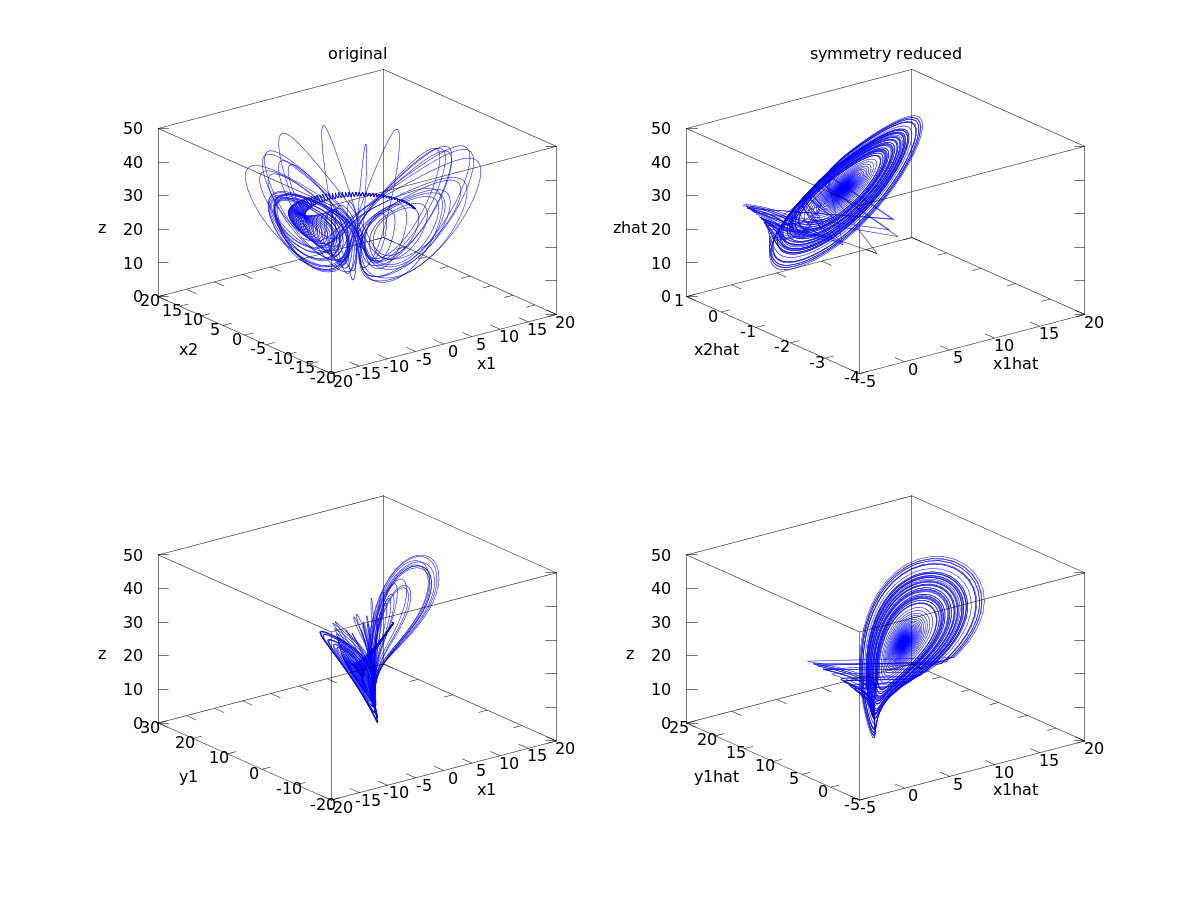
\includegraphics[width=0.9\textwidth]{BBmovingframes}
\end{center}
\caption{ Method of moving frames applied on \cLf.
    }
\label{fig:BBmovingframesCL}
\end{figure}

We can, at least when the symmetry group is abelian, solve the dynamics
on the \reducedsp\ and after that, map it back to the full \statesp\ if
we want to. For the dynamics within the slice, \SOn{2} symmetry we get following
equations:
\bea
  \velRed(\sspRed) &=& \vel(\sspRed) - \dot{\phi} (\sspRed) \groupTan(\sspRed)
\continue
  \dot{\phi}(\sspRed)
    &=& \braket{\vel(\sspRed)}{\sliceTan{}}
    / \braket{\groupTan(\sspRed)}{\sliceTan{}}
\,.
\eea
Here the problem is possibility of getting tangent at the point
$t(\sspRed)$ and the template tangent perpendicular to each other. For
this reason we need multiple, intersecting charts in such a way that this
does not happen. Then we can solve the problem on the
\reducedsp. My unsuccessful attempt of solving reduced dynamics on one
slice:
\end{description}

\begin{figure}[ht]
\begin{center}
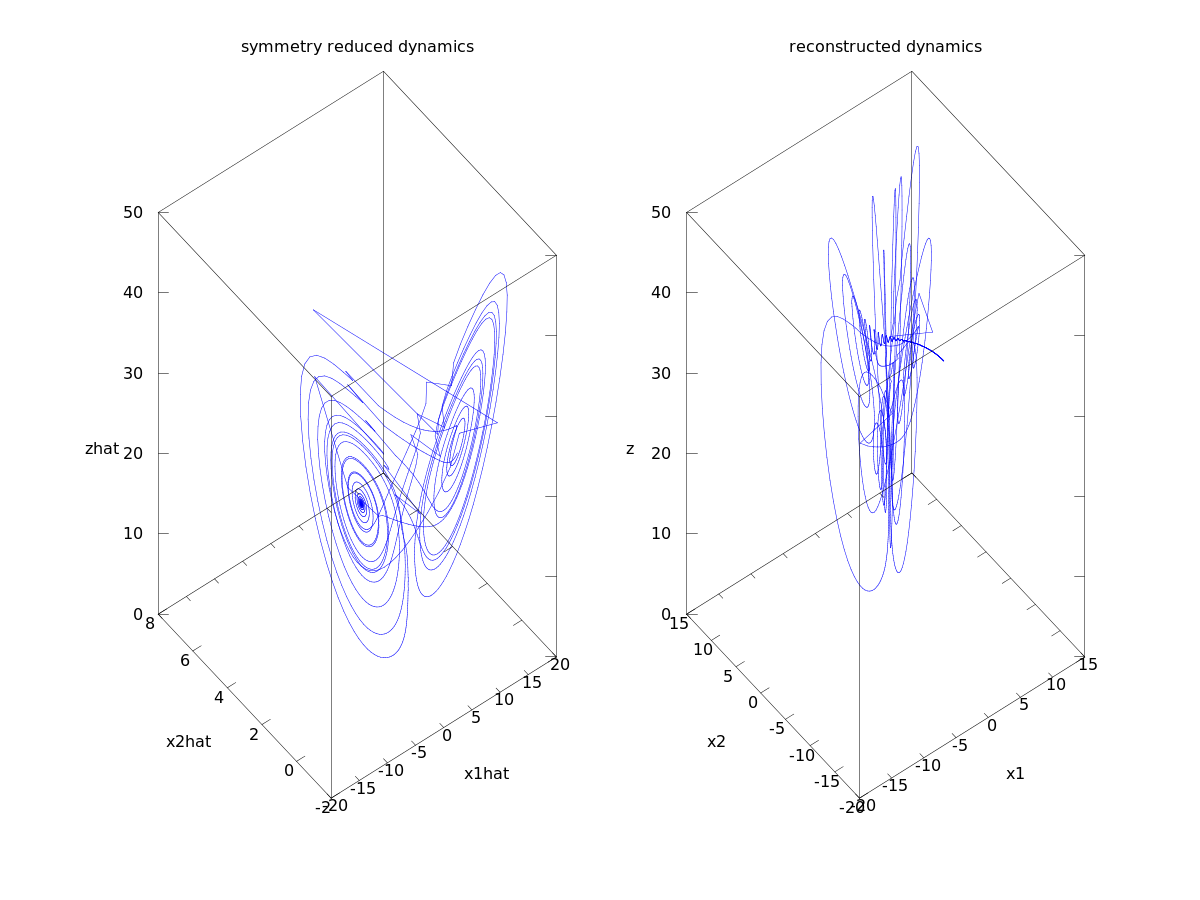
\includegraphics[width=0.9\textwidth]{BBslicedynamics}
\end{center}
\caption{ Dynamics of \cLf\ computed on one slice.
    }
\label{fig:BBslicedynamics}
\end{figure}

\begin{description}

\item[2013-07-25  Predrag]
I have edited your formulas using our macros - it does not matter right
now, but it will be handy later, as one uses different notation for ODE
and PDE \statesp s, for example. One has to be precise about the
language, otherwise one ends up with several things being called `slice',
for example. Definitions are given in Sect.~\emph{V. Charting the slice}
of \refref{atlas12}. A local copy, with all internal comments, is
\HREF{../atlas/atlas12.pdf} {here}.

\refFig{fig:BBmovingframesCL} and \reffig{fig:BBslicedynamics} look
a bit buggy, but basically right.

\item[2013-08-10  Predrag] Moved all Burak's
\twoMode\ $\SOn{2}$-equivariant flow experimentation to file
\texttt{siminos/blog/2modesBB.tex}.

\item[2013-09-11 Daniel] So where are we blogging now? Seems like
stuff is getting moved all over the place... Anyway, while I don't
immediately see an error in Burak's logic, the figure of a single
slice based on the the template (1,1,1,1,0) for \cLf\, seems odd.
When I run my code, I basically get something like figure 4c in the
atlas paper. I haven't run it in a long time so MAYBE I'm doing it
wrong but I think I'm doing it right. Will double check. Looking at
the phase velocity, I get that it gets huge ($\sim$1000). We also
know what the symmetry reduced attractor should look like since
Siminos has studied it in a Hilbert invariant polynomial basis (as
shown in section 10.5 of Das Buch). Both of these things are
single-lobed (with the single-sliced attractor having some
discontinuities), but your figure shows a two-lobed thing. I think
that at one point, we discussed the fact that in the case of \cLf,
just getting to close to the z axis makes the phase velocity blow up,
i.e., you don't actually have to reach the chart border. My
hypothesis at the time was that my cooked up templates for the two
slice atlas worked because they just happened to keep you away from
the z axis as much as possible. That discussion is probably buried
somewhere in the atlas blog.

\item[2013-09-11 Predrag]
\texttt{reducesymm/cgang/2modes.tex} is specific to \twoMode\ article,
\texttt{reducesymm/blog/dailyBlogBB.tex} is about symmetry reduction
in general. It is very awkward to refer to earlier entries in this blog
while sitting in the \twoMode\ article draft.

\item[2013-09-11 Daniel] One last thought that occurred to me on my
way out the door. It is probably nothing but I'll leave it here for
your consideration. Does Burak's argument depend on the fact that
\Lg\ is assumed to have the form that he prescribes. This is not the
most general case, right? For example, \cLf\ is single mode, but
\[
	\Lg =  \begin{pmatrix}
			 0  & 1 & 0 & 0 & 0\\
			 -1 & 0 & 0 & 0 & 0\\
			 0  & 0 & 0 & 1 & 0\\
			 0 & 0 & -1 & 0 & 0\\
			 0 & 0 & 0 & 0 & 0\\
			\end{pmatrix} .
\]

\item[2013-09-11 Predrag] Not sure - but \refeq{eq:LgSO2} is
the form appropriate to \KS\ and pipe flows, so it is worth pursuing.
Anyway, if you read earlier attempts at this slice, it did not work
out for Evangelos and me. Ruslan was happy. The problem is that
unless you can put the 60,000 \KS\ \rpo s into the same slice, I -at
least- have no clue how these solutions are interrelated, and what
the symbolic dynamics might be.

\item[2013-09-11 Burak] My argument is not applicable to the \cLf\ because of the existence of the z coordinate. If one chooses the template as (1,1,0,0,0) as I propose above, when $x_1$ and $x_2$ of \cLf\ becomes zero, the \chartBord\ condition is satisfied regardless of $y_1$, $y_2$ and $z$ values. If you choose (1,1,1,1,0) as the template, then the points which satisfies $\sspRed_1^* = -\sspRed_3^*$ and $\sspRed_2^* = -\sspRed_4^*$  makes the \chartBord , again independent of $z$ coordinate.

\item[2013-09-11 Predrag] Can you read the sections referred to before?
As far as I remember, the first Fourier mode can go through zero, then you need
to fix the second one (at that moment?), etc. Anyway, we could not make it work
in any way that made sense to me.

\item[2013-09-11 Predrag] Wow - I find resolving conflict in git and merging confusing,
svn seems easier. Hope this file is clean now...

\item[2013-09-24 Daniel] Interesting new article by Eckhardt and co.
    entitled \HREF{http://arxiv.org/abs/1309.4590} {Symmetry related
    dynamics in parallel shear flows}\rf{KreEck13}. It's not slicing and
    seems more like the method of connections. Still digesting it but
    will blog about it later.

\item[2013-09-24 Predrag] (unrelated to our \twoMode\ paper, so moved
    to the main blog): If you svn checkout \texttt{pipes}, you'll see our
    discussions: we have sort of written a referee report of
    \refref{KreEck13} already. I still have to discuss the transverse
    diffusion (a result I like) but have lost steam...

\item[2013-10-04 Predrag]
Repository \texttt{svn://zero.physics.gatech.edu/basu} might be of interest.

\item[2013-10-07 Burak] Thanks! It will be helpful.

\item[2013-10-07 Burak] \KS\ equation has an equilibrium at the origin the
corresponding stability matrix is diagonal. Eigenvalues of the first Fourier
mode are positive for the usual choices of system size, which motivates me
for trying my single slice on it. However, I could not manage to produce an
interesting chaotic trajectory by just integrating equations for different
truncations. What I need is a system size parameter ($L$ or $\nu$) and an
initial condition using which I can generate a chaotic orbit with least
number of modes. I looked through the \KS\ literature but could not find
anything helpful. Any suggestions?

\item[2013-10-07 Evangelos] That's funny. I know at least one student in your
group that did his thesis on this problem. I guess it would be hard to spot
his/her publications, so have a look in \refrefs{SCD07,SiminosThesis}.
I would be very interested to see how this first Fourier mode slice works.

\item[2013-10-07 Burak] Already looked at them. Your results are mostly
given in x-space so I need to first digitize, and then Fourier transform
them to be able to use them as initial conditions. You also use at least
16 modes which is something I'm trying to avoid here. I was just asking
if anyone knows an easier way of just getting a chaotic trajectory.

\item[2013-10-07 Evangelos] We played a bit before settling to $L=22$ and,
as we explain in \refrefs{SCD07,SiminosThesis}, this seems to be the smallest
system size for which there is interesting dynamics (or at least you cannot
have a much smaller system that is still chaotic). If you need initial
conditions for \rpo s, there are a lot of them (in Fourier space) in repository
\texttt{siminos}. If you want to simply run a trajectory, then you can start
from any random initial point in Fourier space, just make sure you set
the last few Fourier modes to zero. Computationally, 16 modes are not that many.
Conceptually, it would be better to have something that is 4-d and that's
why we started the PK exercise. However, it turns out that it makes
a great deal of difference in terms of invariant subspaces
when you add a third mode. $L=22$ is interesting because both the second
and the third modes participate in the dynamics. You could try using a smaller
box, but as you have probably seen as you did, there is not much in smaller
systems.


\item[2013-10-03 Evangelos to Burak]
%For the same reason,
What you show in \reffig{fig:BBKSmovframes}, is essentially
equivalent to what we did in our first attempts to reduce symmetry in KS, \ie\
define a slice using the first Fourier mode. See \eg\ Fig. 21.5 in
(svn repository)
\\
\texttt{siminos/blog/blog.pdf}. As you can see we run into
many troubles with this approach, and this led to the atlas (\ie\ multiple chart)
proposal. For instance, in contrast to the {\twoMode} system, KS has no invariant
subspace $a_1=0$, so nothing prevents the flow from crossing the 'chart border'.
I think this is what you see in your figure, and refined numerical integration
will not help.

\item[2013-11-04 Burak to Evangelos] To show that higher time resolution
smoothes the discontinuities I sampled the solution with a higher rate and
applied the same symmetry reduction.  You can see that \reffig{fig:BBKSmovframes}(b)
does not have the annoying jumps of \reffig{fig:BBKSmovframes}(a), only difference
in the production of the two is the spacing between time samples.

I'll try to explain the magic by writing the slice and chart border conditions
and rotations explicitly for different cases. If we define $Re[a_1] = x_1$ and
$\Im[a_1] = y_1$, $\SOn{2}$ operation on these coordinates yields
\bea
	\hat{x}_1 &=& \cos{\phi} \, x_1 + \sin{\phi} \, y_1
	\continue
	\hat{y}_1 &=& - \sin{\phi} \, x_1 + \cos{\phi} \, y_1 \, .
	\label{eq:SO2on1stmode}
\eea
Let's take the \template\ as $\slicep = \{0,1\}$. For this template, \slice\
condition is
\beq
	\hat{x}_1 = 0 \, ;
	\label{eq:SliceCondIma1}
\eeq
and the \chartBord\ is defined by
\beq
	\hat{y}^*_1 = 0 \, .
	\label{eq:ChartBordIma1}
\eeq
Substituting \refeq{eq:SliceCondIma1} in \refeq{eq:SO2on1stmode}, we get
\bea
	0 &=& \cos{\phi} \, x_1 + \sin{\phi} \, y_1 \rightarrow\ x_1 = - \frac{\sin{\phi}}{\cos{\phi}} y_1 ,
	\continue
	\hat{y}_1 &=&  \sin{\phi} \, \frac{\sin{\phi}}{\cos{\phi}} y_1 + \cos{\phi} \, y_1 \, \rightarrow\ \hat{y}_1 = \frac{y_1}{\cos{\phi}} \, .
	\label{eq:SO2on1stmodeIma1}
\eea
We see that, whenever the flow crosses $\Im[a_1] = 0$ we cross the \chartBord,
which is something frequently happens in both \KS\ and \twoMode\ systems. You
would get a similar condition if you had choosen the \template\ as $\slicep = \{0,1\}$.
\BBedit{(FALSCH. SEE [2013-11-18 Burak] FOR CORRECTION.)}

Now let's take the \template\ $\slicep = \{1,1\}$. For this one, \slice\
condition is
\beq
	\hat{x}_1 = \hat{y}_1 \, ;
	\label{eq:SliceConda1}
\eeq
and the \chartBord\ is defined by
\beq
	\hat{x}^*_1 = \hat{y}^*_1 = 0 \, .
	\label{eq:ChartBorda1}
\eeq
You can easily see by following the same steps that only the solutions with
$x_1 = y_1 = 0$ are mapped to the \chartBord\ defined by \refeq{eq:ChartBorda1}.
This condition is much more restrictive than the previous one. It is not allowed
in \twoMode\ case by the fact that it is in an invariant subspace and I, myself,
haven't encountered that in \KS\ solutions; other than the \rpo s with fundamental
frequencies of second or third mode.

In addition to my strong belief that it is extremely unlikely to have a zero
magnitude 1st mode, I am almost sure that you cannot cross the \chartBord\
\refeq{eq:ChartBorda1} since in the \mframes\ you make a direction choice
which restricts the \reducedsp\ to a half space in which $\Re[a_1]$
is either greater or lesser than $0$ for the choice $\slicep = \{1,1,0,0,\cdots\}$,
hence, the worst you can do is to touch the \chartBord\ and come back to safety.
You can see this on \reffig{fig:BBKSmovframes}. In \reffig{fig:BBKSmovframes},
the direction choice resulted $Re[\hat{a}_1]$ being lesser than 0 and the
projection of the \chartBord\ is the plane $Re[\hat{a}_1] = 0$. The flow
gets close to that but never crosses it.

Regarding your former discussions, I'm totally on Ruslan's side. I think the
smallest non-vanishing Fourier mode is the most natural basis for the symmetry
reduction of an equation defined on a periodic domain.

I would be convinced that what I am suggesting here is no better than what
you tried before if you show me an example of a \KS\ solution that crosses
$|a_1| = 0$.

\item[2013-11-18 Burak]
Found an error in my interpretation of equation \refeq{eq:SO2on1stmodeIma1}.
For a point $(x_1, y_1) = (x_1, 0)$, the mapping onto the slice is satisfied
by picking the group parameter as $\phi = \pi / 2, 3 \pi / 2,...$. So taking
the relation $x_1 = - (\sin{\phi}/\cos{\phi})y_1$ and plugging in to the next equation
was not a right thing to do. If you plug in $\phi = \pi/2$ in each equation in
\refeq{eq:SO2on1stmodeIma1} you get $(\hat{x}_1, \hat{y}_1) = (0, x_1)$ and
the tangent is parallel to the template tangent. Hence all the 1st mode slices
are equivalent as geometry suggests. However, it's still true that the \chartBord\
is at $x_1 = y_1 = 0$ for the 1st slices hence it's at the point where the slice
ends.

\item[2013-11-08  Predrag]
Refereed Marina Pausch, Florian Grossmann, Bruno Eckhardt, and Valery
G. Romanovski\rf{PGER13} {\em Gr{\"o}bner basis methods for stationary
solutions of a shear flow}
(\HREF{http://ChaosBook.org/library/PGER13.pdf}{click here}). Bruno
seems to get on every plumbing paper published. This might be of
interest to Burak, as they write: ``Even though systems of
multivariate polynomials are pervasive in all areas of applied
science and engineering, no algorithmic methods to solve such systems
were known until the mid-sixties of the last century, when Bruno
Buchberger invented the theory of Groebner bases. They have since
become the cornerstone of modern computational algebra.''


I wrote to authors:
``I find this application of the Gr{\"o}bner basis methods to search for
equilibrium solutions for a model of a fluid flow very interesting,
and a useful reference for what is known about polynomial methods.
Traditionally, one searches for Navier-Stokes solutions using
Newton-Raphson methods, and has no clue as to whether one has found
all solutions.''

I wrote to (confidential comment) to editor:
`` I am not an expert on the Gr{\"o}bner basis methods, so hope you do
get an expert opinion. I have not gone through the paper in any
detail. However, I am interested in finding equilibrium solutions for
Navier-Stokes flows, and I find this paper a useful reference to what
is known about polynomial methods (we search for solutions using
Newton-Raphson methods, and have no clue as to whether we have found
all solutions). I recommend that paper be published. ''

\item[2013-11-18 Predrag to Valery Romanovski] (Maribor)
Posted the day's draft of \texttt{2modes.pdf}. Asked: ``Is there an
elegant, systematic way of finding roots of such bivariate polynomials? A
simple example of your multivariate polynomial methods? I would like to
include the important references to this literature in ChaosBook.org.''

\item[2013-11-20 Valery Romanovski]
I do not know something special about solving systems of 2 bivariate
polynomials. Practically it is not too difficult (if you have 2-3
parameters). You just compute the resultant or a Gr{\"o}bner basis with
respect to a lex order reducing the problem to finding roots of an
univariate polynomial and then find roots of  this polynomial.

If you have many parameters then, I believe, it is difficult to find
distribution of number of roots in the parameter space.

By the way, I had a look at your system (18) on page 4. Is it interesting
for you to find some values of parameters for which the system has
invariant hypersurfaces and some values of parameters for which  it
admits integrals? I have some methods to look for such objects in
polynomial systems.

\item[2013-11-21 Predrag] Been reading
\HREF{http://mathworld.wolfram.com/GroebnerBasis.html} {wolfram.com}
which has a link to Buchberger's ``Groebner Bases: A Short Introduction
for Systems Theorists.'' I started a file which generates 8th order
polynomial in $u$ which presumably generates all roots, but have not
finished (the polynomial is huge) - it's in
\texttt{mathematica/Groebner.nb}. Mentioned I was doing it to UFO - he knew
about Buchberger. Seems to know everything.

\item[2013-11-12 Burak]
I added the abstract for Dynamics Days in
\\
\texttt{blog/burak/DynamicsDays/twomodeabstract.tex}.

\item[2013-11-18 Predrag to Burak] Chairman Ruslan's epicycles,
worth rereading:
\refsect{HowtoQuotSO2}, \refsect{HowtoSliceSO2};
\HREF{davidchack/071231fundamental.html}
{siminos/blog/davidchack/071231fundamental.html}.

\item[2006-09-03 Ruslan]
KS \eqva\ discussion:
\\
\HREF{http://www.math.le.ac.uk/people/rld8/temp/kse22explore.html}
{www.math.le.ac.uk/people/rld8/temp/kse22explore.html}
\\
There is much more, just search for Ruslan throughout this blog.

Now that you are looking at the unstable manifold of $\REQV{\pm}{1}$, it
would be good to (re)read Chapter VIII of Siminos thesis.

\item[2014-04-23 Burak] I started reviewing QFT in my free time and looked
at the $\phi^4$ equations of motion, which is a nonlinear PDE:
\beq
	(\partial^2 + m^2) \phi = - \frac{ \lambda}{3!} \phi^3 .
\eeq
I then googled for the numerical solutions of Klein-Gordon equation and
found some literature. Wikipedia article has some
\HREF{http://en.wikipedia.org/wiki/Klein\%E2\%80\%93Gordon_equation\#Traveling_wave_solution}{
travelling wave solutions}. If 1D equation gives anything interesting, it
could be solved and sliced by changing a few lines in my \KS\ code. For now,
I'm just taking a note here that this could be a candidate for slicing.
\end{description}

% former siminos/ksRecycled/tex/blog.tex    master file: BuDiCv15.tex
%%%%%%%%%%%%%%%%%%%%%%%%%%%%%%%%%%%%%%%%%%%%%%%%%%%%%%%%%
% \section{Burak's BuDiCv15 blog} \label{sect-BuDiCv15blog}
\input BuDiCv15blog
% Predrag 2016-03-28 brought here  BuDiCv15 blog
%%%%%%%%%%%%%%%%%%%%%%%%%%%%%%%%%%%%%%%%%%%%%%%%%%%%%%%%%

\renewcommand{\ssp}{a}
